
\chapter{\label{chapter5_normToLeuk}A regulatory network driving MLL-AF9 GMP leukaemogenesis}
\chaptermark{Chapter 5 - MLL-AF9 GMP GRN}

\begingroup
\raggedright
\minitoc
\endgroup

% Put declaration here?!

\clearpage{}
\section{\label{ch5:mre-intro}Introduction and aims}

\begin{wrapfigure}{r}{0.5\textwidth}
  \begin{center}
    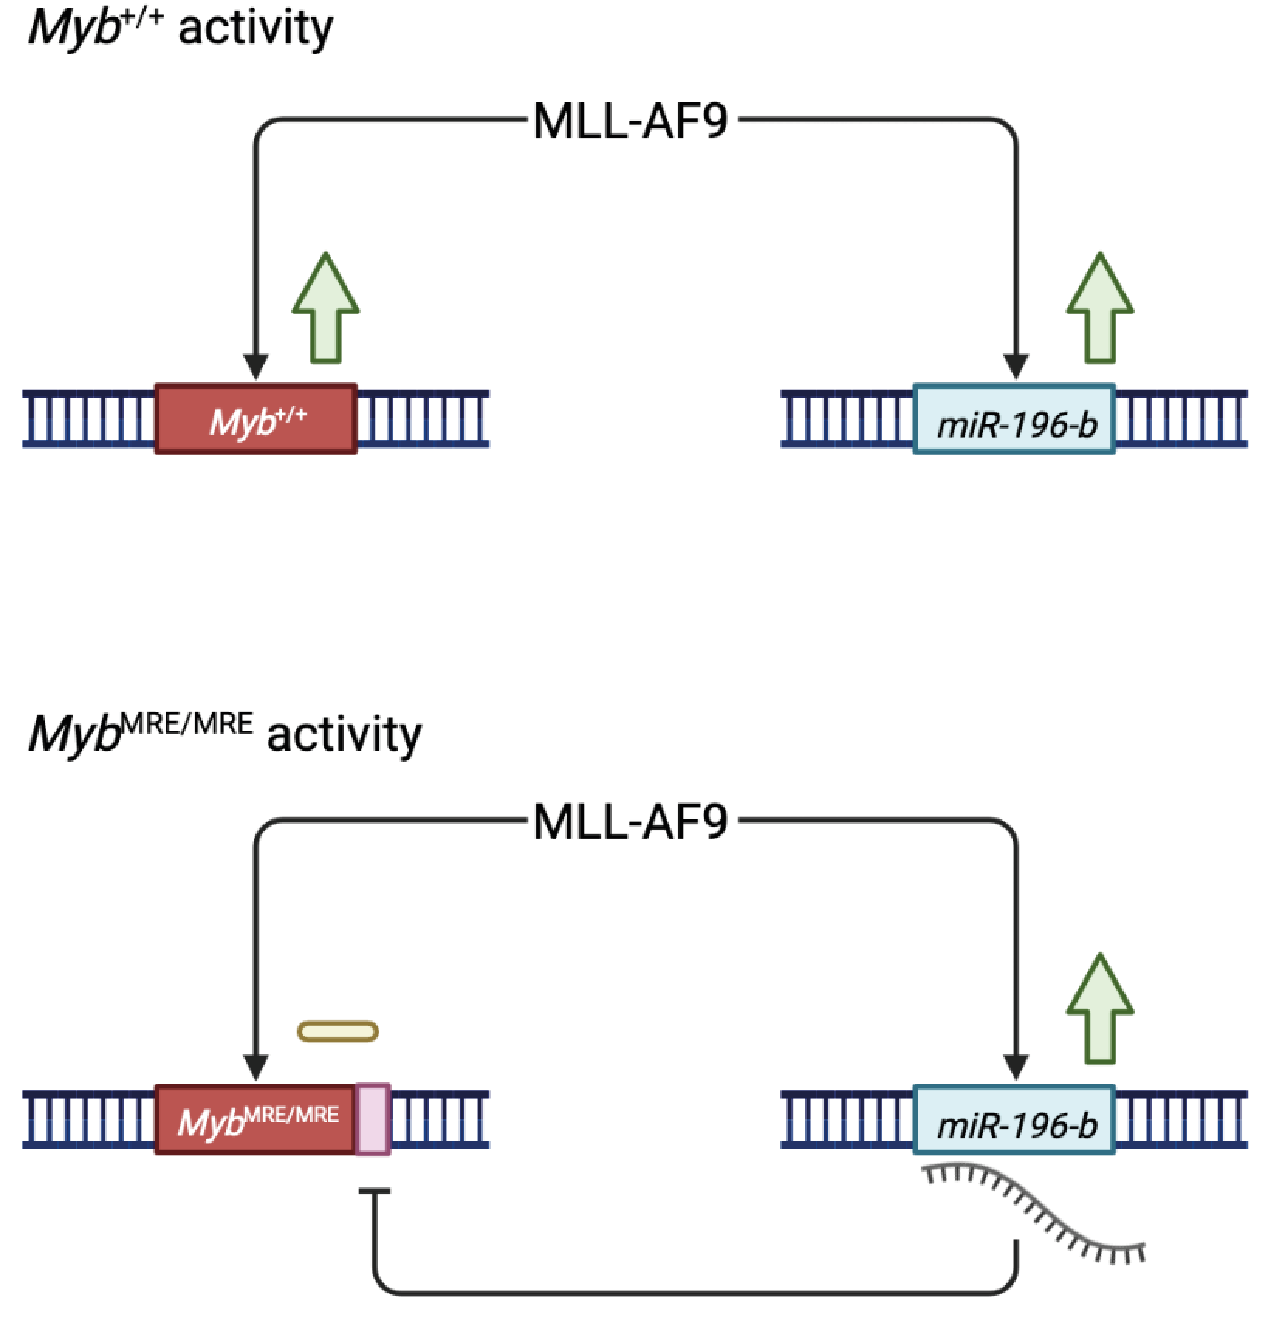
\includegraphics[width=0.48\textwidth]{figures/chapter5/ch5_mre-intro.png}
  \end{center}
  \caption[{Schematic of \mybmre{} engineered circuit.}]
    {\textbf{Schematic of \mybmre{} engineered circuit.} 
    Schematic illustrating \mybwt{} and \mybmre{} genotypes, and the action of MLL-AF9 in these contexts. \mybmre{} includes a \textit{miR-196b} response element in the 3' UTR of \textit{Myb}, resulting \textit{miR-196b} repression of \textit{Myb}. As MLL-AF9 drives both \textit{miR-196b} and \textit{Myb} expression, this acts to intrinsically repress \textit{Myb} activity during leukaemogenesis. 
    \textit{\mybmre{} mouse models designed and generated by I. Lau \citep{lau_role_2022}. Figure created with BioRender.com.}
    }
    \label{fig:ch5_mre-intro}
\end{wrapfigure}

In chapters 3 and 4, I established and analysed GRN models describing aspects of normal and aberrant haematopoiesis. This involved a model of EHT, the process underlying the embryonic origin of HSCs, and a model of MLL-AF4 leukaemia. The MLL-AF4 GRN represented a steady state system, where the leukaemia has already progressed significantly. For this next chapter I have attempted to model early stages of leukaemogenesis, alongside conditional perturbation of the critical TF Myb in the presence of MLL-AF9, using a system previously established by I. Lau \citep{lau_role_2022}. This system involves the transduction of mouse granulocyte-monocyte progenitors (GMPs) with human MLL-AF9, and expansion of these cells in MethoCult. MLL-AF9 is known to activate \textit{Myb}, which is then required for leukaemia maintenance \citep{zuber_integrated_2011}. MLL-AF9 also upregulates the micro-RNA (miRNA) \textit{miR-196b} \citep{popovic_regulation_2009}, which as a miRNA results in downstream gene repression \citep{huntzinger_gene_2011}. Previous work by I. Lau generated an engineered mouse model where two \textit{miR-196b} miRNA response elements (MREs) were inserted into the 3' UTR of \textit{Myb} \citep{lau_role_2022}, resulting in a conditional circuit where upon MLL-AF9 induction of \textit{miR-196b}, \textit{Myb} is targeted for repression (Fig. \ref{fig:ch5_mre-intro}). In this chapter I have established a GRN model using both \mybwt{} and \mybmre{} mice, combined with MLL-AF9 transduction of GMPs, to describe early transcriptional adaptations to \textit{MLL-AF9} expression. As this \mybmre{} conditional model was constructed to perturb \textit{Myb}, I have focused the analysis of this chapter on the role of Myb in MLL-AF9 leukaemia.

The GRN models in chapters 3 and 4 were constructed using different methodologies, with advantages and disadvantages to each approach. The EHT model involved a thorough dissection of gene expression and chromatin accessibility patterns, integrated through motif detection. While this established a broad set of potential regulators, it lacked physical evidence of TF binding. The MLL-AF4 GRN instead relied on ChIP-seq data to identify regulatory interactions, and used perturbation data to focus the GRN on specific protein behaviours. It relied heavily on cell line models, which are poor representations of real patient biology. While this resulted in a robust and targeted GRN, the wider network was less reliable as the motif data was sourced from published deepCAGE data based on THP-1 cells, and there were not enough samples to perform correlation analyses. Going forward, to establish a GRN using this \mybmre{} model, I took lessons learned from chapters 3 and 4 to build a more complete network model. The aim was to establish a GRN that incorporates a time course, gene expression correlation, TF binding motifs, RNA-seq, ATAC-seq and ChIP-seq data, and perturbation data through the \mybmre{} mouse model. This will allow the generation of a robust network that can be used to probe the role of Myb as GMP regulatory networks adapt to the presence of MLL-AF9 over time, as a model of leukaemogenesis. 

\noindent
\textbf{Aims}

\vspace*{-5mm}
\begin{enumerate}
    \item To characterise transcriptional and epigenetic adaptations to human \textit{MLL-AF9} expression in GMPs. 
    \item To establish a GRN model of GMP leukaemogenesis over time.
    \item To investigate the impact of \textit{Myb} perturbation in the MLL-AF9 leukaemogenesis model.
\end{enumerate}

\vspace*{-5mm}
The addition of MLL-AF9 to normal mouse GMPs allows the characterisation of MLL-AF9 leukaemogenesis and the construction of a GRN model that incorporates a time course experiment. This GRN model will highlight how regulatory circuits adapt over time to \textit{MLL-AF9} expression. Further, by including a \mybmre{} mouse system, \textit{Myb }perturbation data is incorporated in the model, allowing for specific questions on TF behaviour in the context of leukaemogenesis.

\clearpage
\section[Experimental design to characterise MLL-AF9 GMP leukaemogenesis]{\label{ch5:MethoCult}Experimental design to characterise\\MLL-AF9 GMP leukaemogenesis}

\begin{figure}[!b]
    \centering
    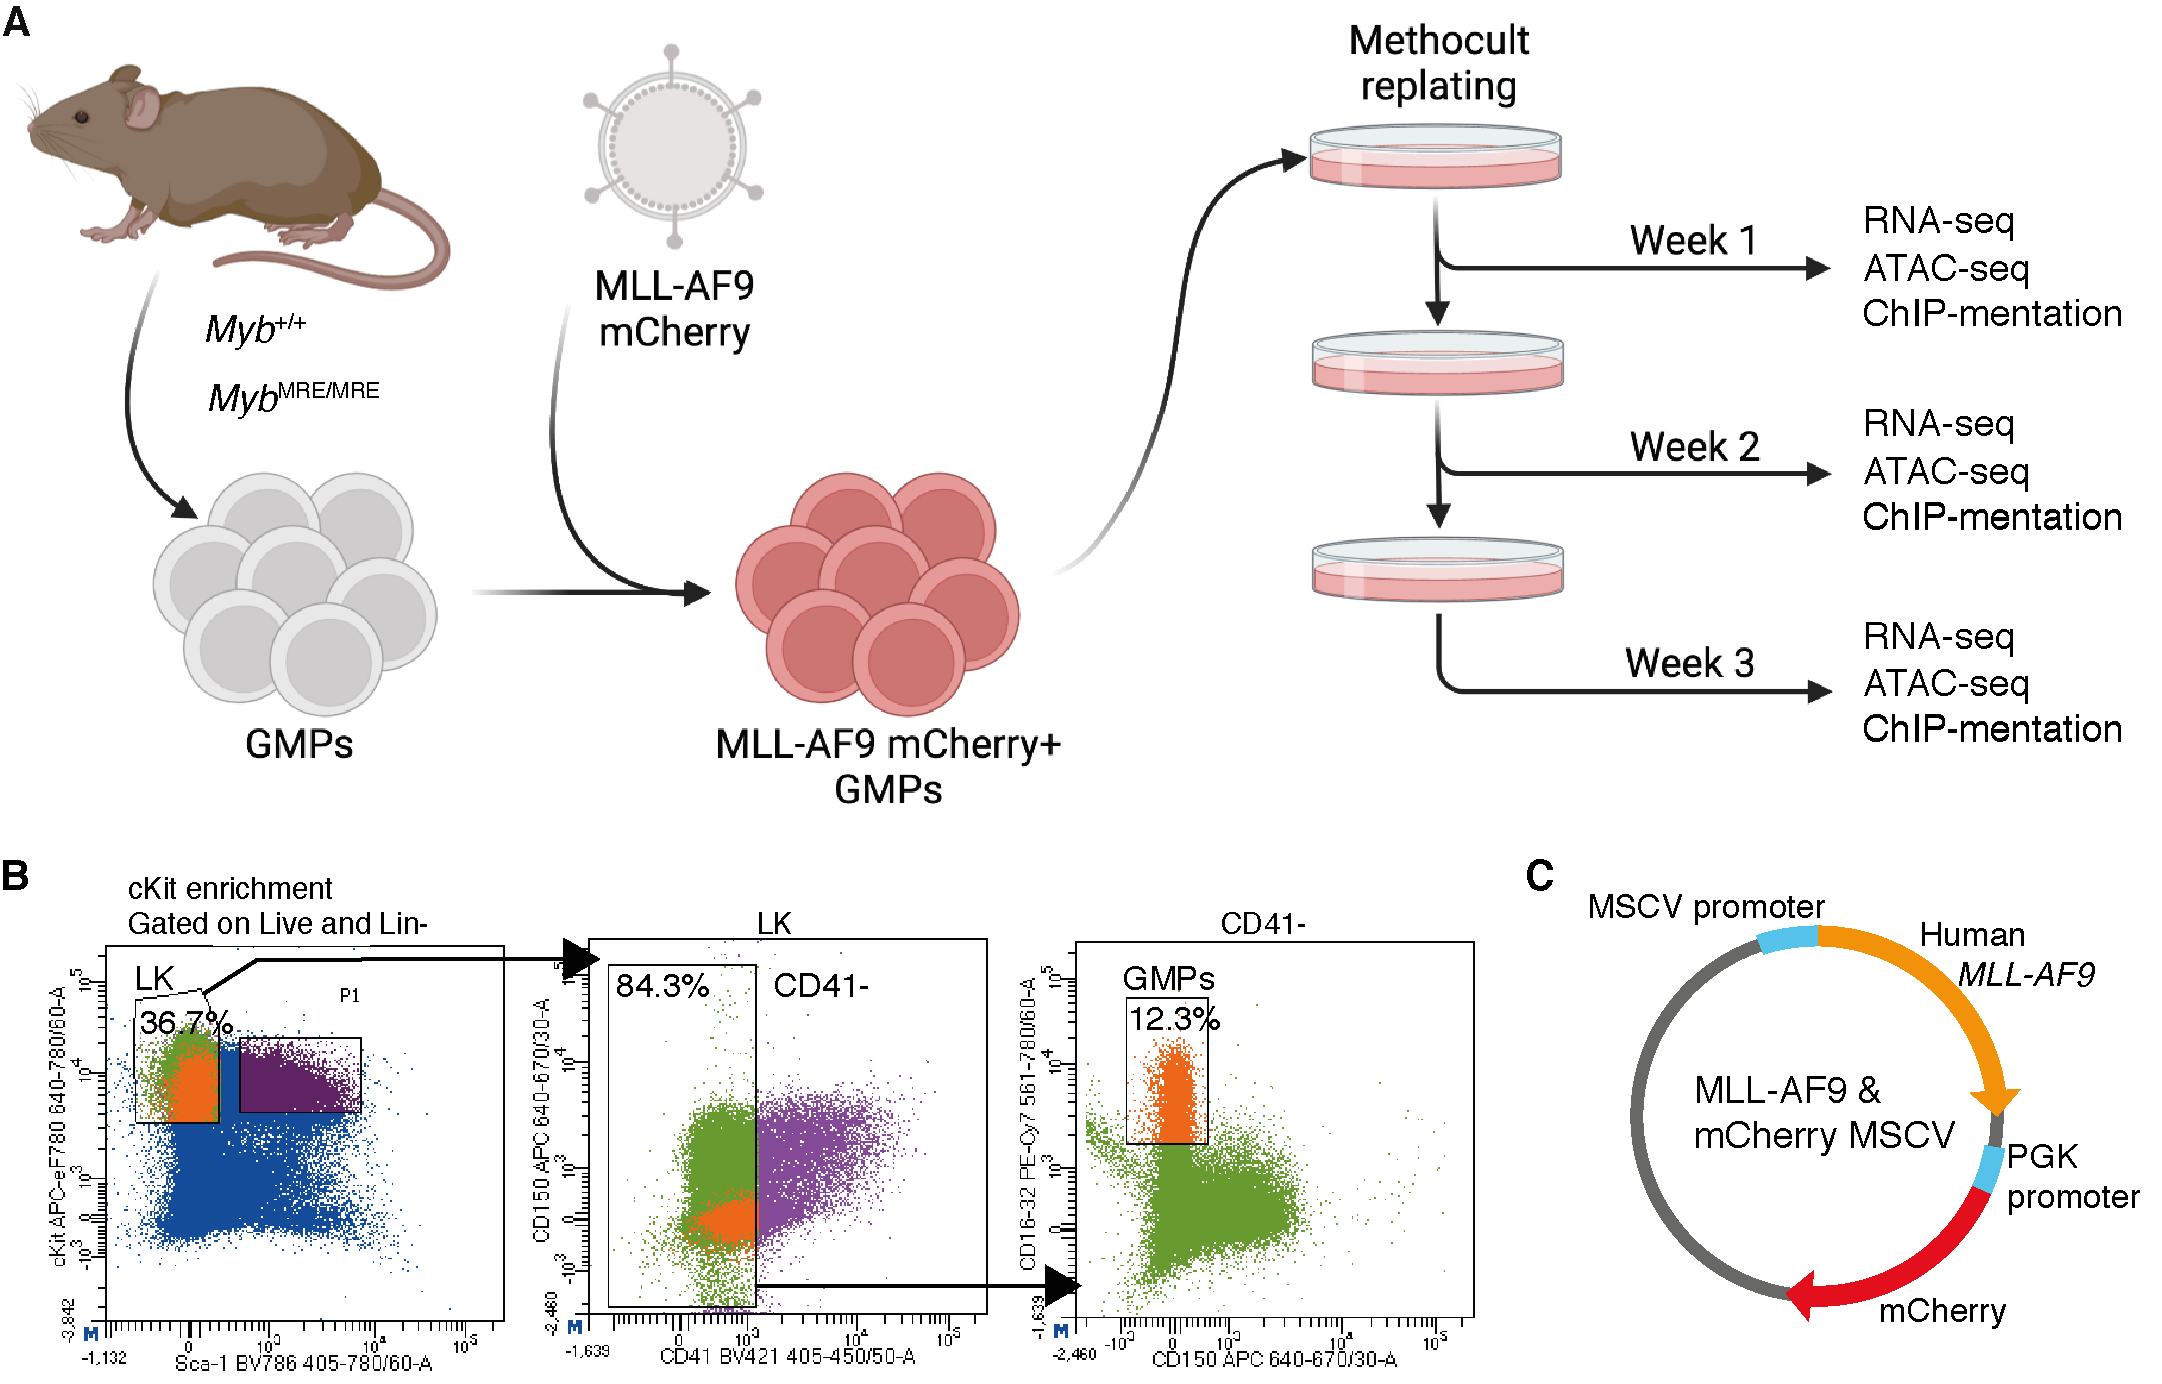
\includegraphics[width=\textwidth,height=\textheight,keepaspectratio]{figures/chapter5/ch5_overview.png}
    \caption[{Experimental plan for MLL-AF9 transformation of GMPs and MethoCult expansion.}]
    {\textbf{Experimental plan for MLL-AF9 transformation of GMPs and MethoCult expansion.}
    \textbf{(A)} Schematic overview for plan to virally transduce mouse GMPs with a human MLL-AF9:mCherry construct and expand in MethoCult. Cells were replated in MethoCult each week. 
    \textbf{(B)} Representative sort gates for isolation of GMPs from mouse bone marrow. c-Kit positive cells were isolated by magnetic bead purification before staining and flow cytometry. LK: Lin-cKit+. 
    \textbf{(C)} Illustration of MSCV MLL-AF9:mCherry plasmid, with human \textit{MLL-AF9} and \textit{mCherry} constitutively active under the MSCV and PGK promoters, respectively. 
    \textit{Experimental design adapted from I. Lau, and MSCV MLL-AF9:mCherry construct generated by I. Lau \citep{lau_role_2022}. Panel A created with BioRender.com. }
    }
    \label{fig:ch5_overview}
\end{figure}

To address how MLL-AF9 causes transcriptional and epigenetic adaptations over time, I established an experimental design to construct a GRN model incorporating multiple time points following \textit{MLL-AF9} expression (Fig. \ref{fig:ch5_overview}A). GMPs were isolated from mouse bone marrow as Lin\uneg{}cKit\upos{}CD41\uneg{}CD150\uneg{}CD16/32\upos{} (Fig. \ref{fig:ch5_overview}B), as in \cite{pronk_elucidation_2007}. GMPs were retrovirally transduced with a construct containing human \textit{MLL-AF9} expressed from the Murine Stem Cell Virus (MSCV) promoter and an \textit{mCherry} fluorescent marker expressed from the 3-phosphoglycerate kinase (PGK) promoter (Fig. \ref{fig:ch5_overview}C). After 24 hours' incubation, mCherry+ GMPs were sorted directly into MethoCult. mCherry+ GMPs were expanded in MethoCult for three weeks with replating each week. Every week (W1-3) cells were collected for RNA-seq (\xten{5}{5} cells), ATAC-seq (\xten{1}{5} cells), and ChIPmentation (\xten{7}{5} cells) (Fig. \ref{fig:ch5_overview}A). ChIPmentation was performed instead of ChIP-seq due to the limited cell numbers. This experiment was performed in parallel using GMPs sourced from both \mybwt{} and \mybmre{} mice, to allow comparisons between normal \textit{Myb} activity and conditional \textit{Myb} perturbation, and was performed in triplicate.

Maintenance of \textit{MLL-AF9} expression after expansion in MethoCult was confirmed by RT-PCR, using primers targeting human MLL-AF9 (Fig. \ref{fig:ch5_MethoCult-validation}A), and the genotypes of \mybwt{} and \mybmre{} samples were validated (Fig. \ref{fig:ch5_MethoCult-validation}B). As noted by I. Lau \citep{lau_role_2022}, the \mybmre{} genotype should confer reduced colony forming potential. In this experiment, by W3 \mybwt{} samples showed considerably more colonies (Fig. \ref{fig:ch5_MethoCult-validation}C), although colony counting was only performed for two replicates. 

\begin{figure}[!h]
    \centering
    \includegraphics[width=\textwidth,height=\textheight,keepaspectratio]{figures/chapter5/ch5_MethoCult-validation.png}
    \caption[{MLL-AF9 GMP replating validation.}]
    {\textbf{MLL-AF9 GMP replating validation.}
    \textbf{(A)} PCR validation using cDNA from W3 MLL-AF9 GMPs showing MLL-AF9 expression (667 bp product). mESC and THP-1 cDNA used as negative and positive controls, respectively. O'GeneRuler 1Kb+ used for size ladder. 
    \textbf{(B)} PCR validation using cDNA from W3 MLL-AF9 GMPs to confirm \textit{Myb} genotypes. PCR products indicate \mybwt{} at 186 bp and \mybmre{} at 233 bp. O'GeneRuler 1Kb+ used for size ladder. 
    \textbf{(C)} Total colony counts in MethoCult over three weeks of culture and replating. Week 1 counts were over one plate, while weeks 2 and 3 were counted over three plates per replicate. \textit{n} = 2. 
    }
    \label{fig:ch5_MethoCult-validation}
\end{figure}
\clearpage

I performed the RNA-seq, ATAC-seq and ChIPmentation library preparation of the transformed cells at each time point. ChIPmentation was performed using antibodies raised against MLL-N, H3K27ac, and H3K4me1. Typical RNA Tapestation traces showed high quality RNA (Appendix \ref{fig:app_methocult-tapestation}), with intact 18S and 28S ribosomal RNA peaks, and library prepped samples showed expected fragment sizes. ATAC-seq samples showed clear mono- and di-nucleosome fragments (Appendix \ref{fig:app_methocult-tapestation}). After sequencing, RNA-seq and ATAC-seq samples showed a high number of PCR duplicates (RNA-seq: 37.15\% - 67.22\% PCR duplication, with mean of 59.75\%. ATAC-seq: 28.27\% - 52.67\% PCR duplication, with mean of 40.2\%) (Appendix \ref{fig:app_methocult-qc}A-B). ChIPmentation samples had low read counts (\xten{6.09}{6} - \xten{1.35}{7} read counts, with mean of \xten{9.64}{6}) with few PCR duplicates (7.95\% - 28.03\% PCR duplication, with mean of 14.31\%) (Appendix \ref{fig:app_methocult-qc}C), suggesting that the ChIPmentation samples could be sequenced more deeply to increase complexity. After PCR deduplication, all samples were mapped successfully (Appendix \ref{fig:app_methocult-qc}A-C). Overall, these quality control measures showed the data was of a reasonable quality for analysis. 

\section{\label{ch5:profiles}Gene expression and chromatin accessibility adapts over time, while MLL-AF9 binding is stable.}

\begin{figure}[!t]
    \centering
    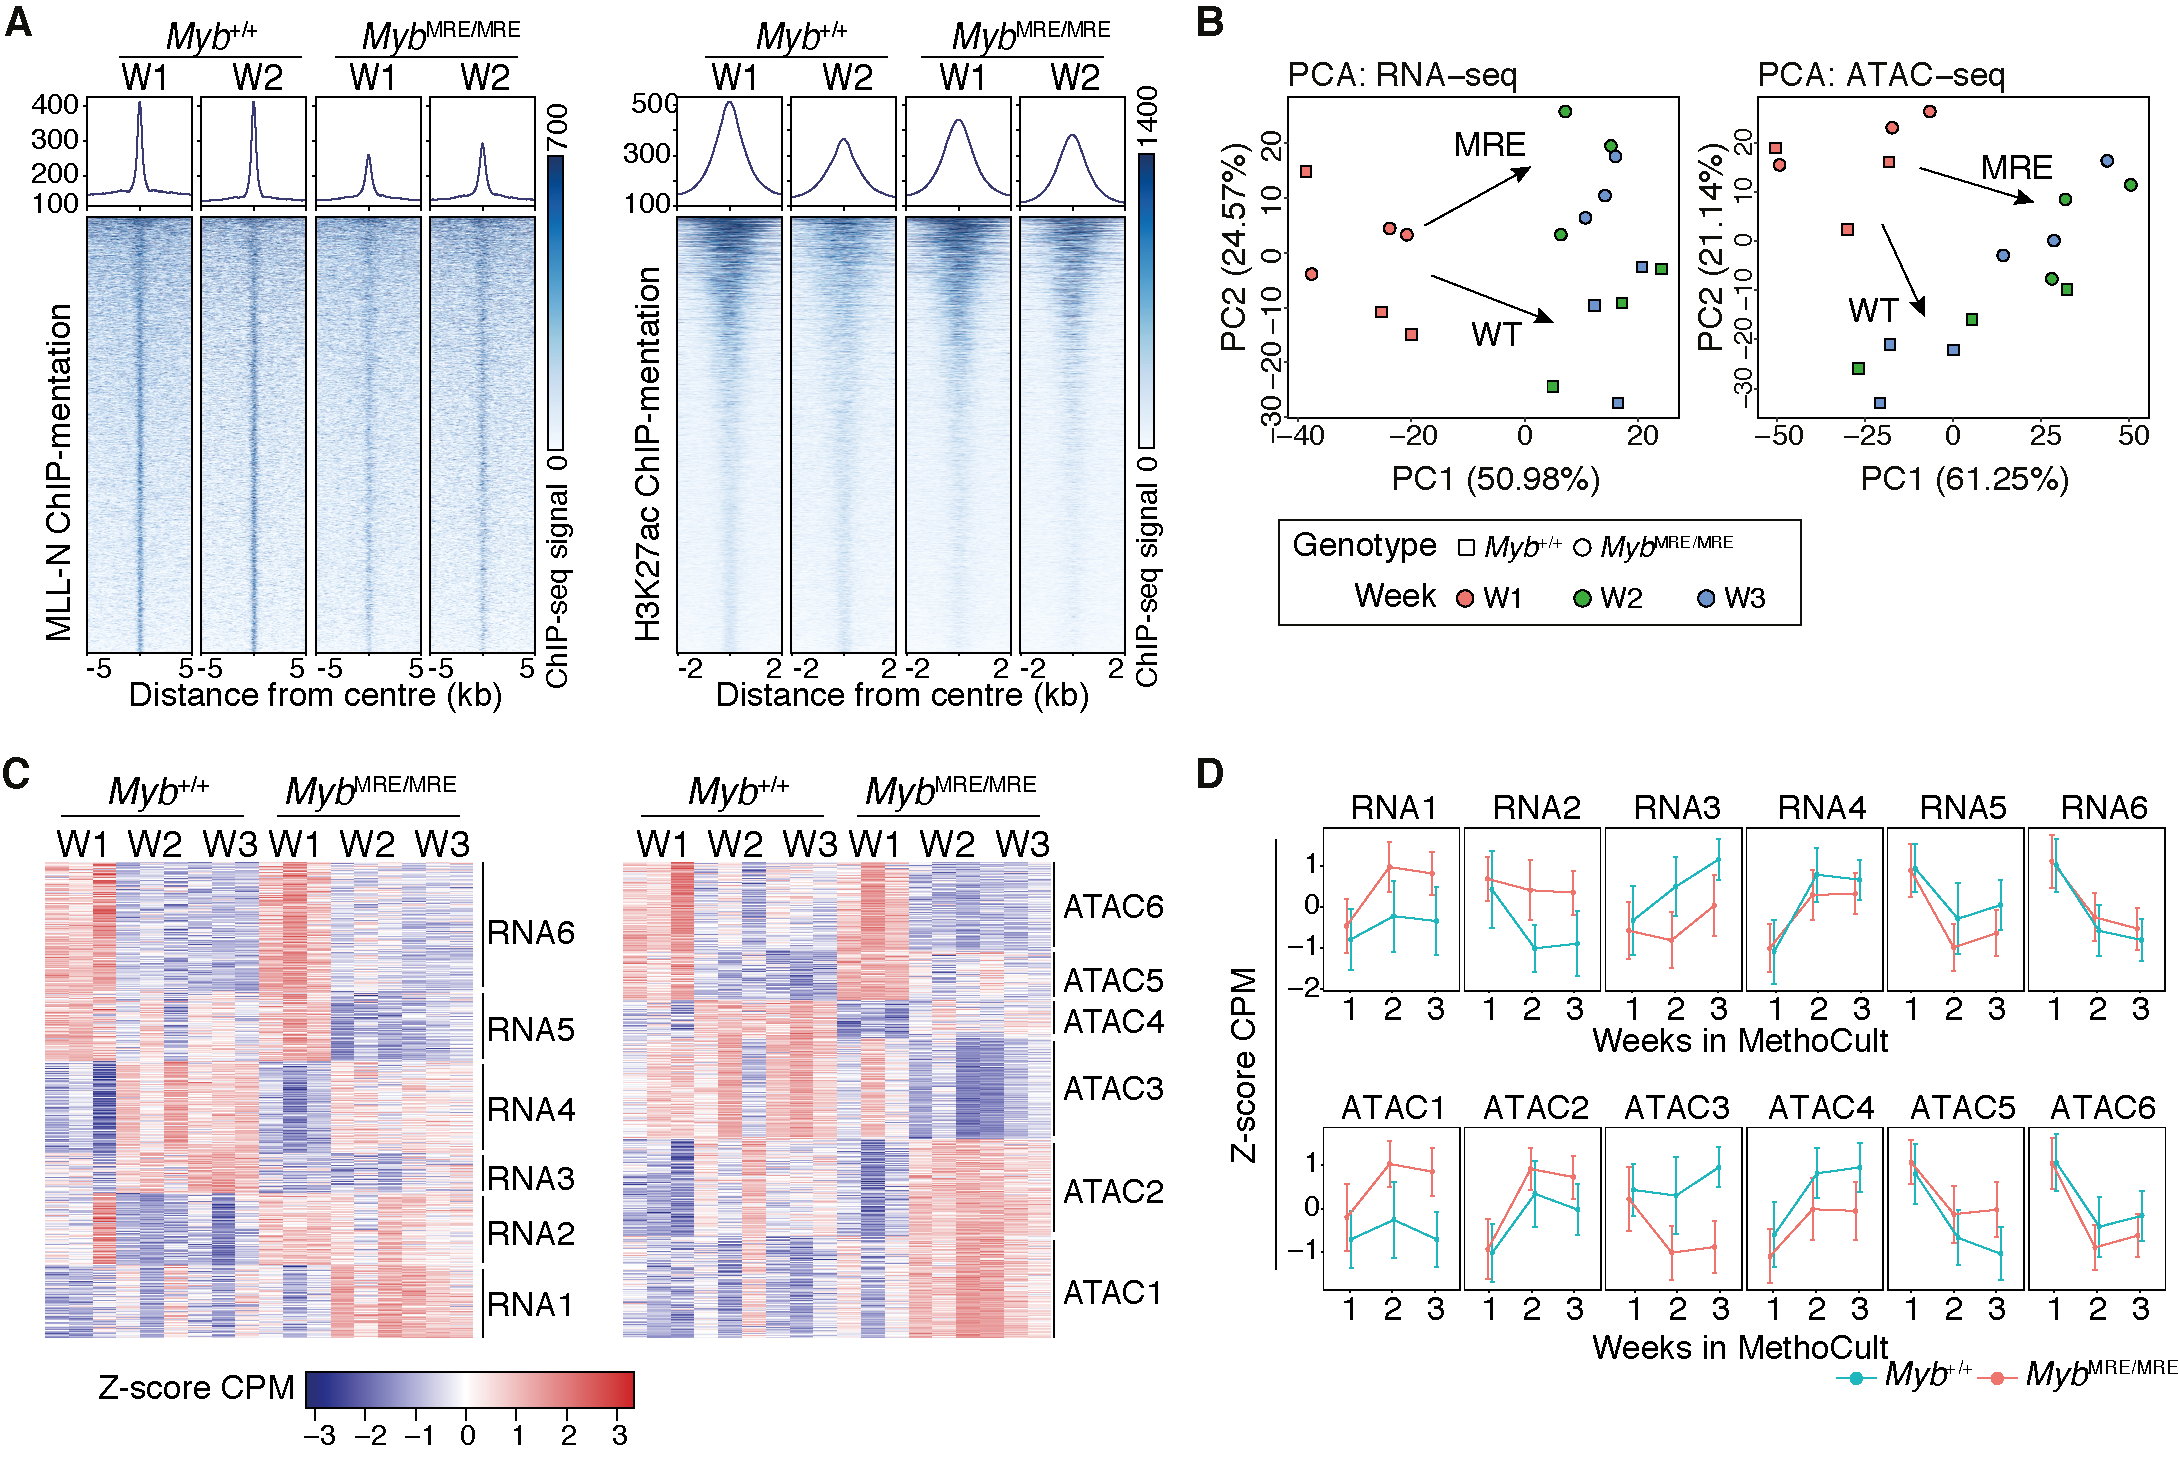
\includegraphics[width=\textwidth,height=\textheight,keepaspectratio]{figures/chapter5/ch5_profiles.png}
    \caption[{RNA and chromatin accessibility adapts from W1 to W2/3, yet MLL-N profiles are stable by W1.}]
    {\textbf{RNA and chromatin accessibility adapts from W1 to W2/3, yet MLL-N profiles are stable by W1.}
    \textbf{(A)} MLL-N and H3K27ac ChIPmentation heatmaps in W1 and W2 MLL-AF9 transformed GMPs, at MLL-N peaks (left) and H3K27ac peaks (right), ordered by ChIPmentation signal. MLL-N peak calls were performed on combined W1 and W2 data. Metaplots showing average signal shown above.
    \textbf{(B)} PCA plots of RNA-seq (left) and ATAC-seq (right) samples, with ANOVA DEG and DAEs used as inputs. \textit{Myb} genotypes represented by data point shape. Arrows indicate transition from W1 to W2 and W3 samples, for \mybwt{} and \mybmre{}.
    \textbf{(C)} Expression and accessibility heatmaps (z-score log\textsubscript{2} CPM) for RNA-seq DEGs  (left) and ATAC-seq DAEs (right). Genes and peaks grouped by \textit{k}-means clustering into modules. 
    \textbf{(D)} Average z-score log\textsubscript{2} CPM of gene expression (top) and chromatin accessibility (bottom) by modules as in C. Bars indicate standard deviation of the mean.
    }
    \label{fig:ch5_profiles}
\end{figure}

To determine the MLL-AF9 binding pattern over time, MLL-N ChIPmentation was summarised over MLL-N peak calls (Fig. \ref{fig:ch5_profiles}A). Interestingly, MLL-N signal is present at similar levels and distribution between W1 and W2, suggesting that MLL-AF9 binding profiles do not change over the time course. In comparison to \mybwt{}, the \mybmre{} samples, despite showing similar binding profiles, indicate reduced MLL-N binding. H3K27 acetylation shows a similar distribution of signal between W1 and W2, but with reduced levels at W2, for both genotypes. Note that the ChIPmentation samples are somewhat under-sequenced, and have not been reference normalised, so these observations are not fully robust. However, this analysis suggests that MLL-AF9 binding does not significantly change over time, though there may be differences between \mybwt{} and \mybmre{} genotypes. In contrast, H3K27 acetylation appears to decrease over the time course, suggesting changes in the chromatin environment.

To address whether gene expression or chromatin accessibility profiles change during MethoCult expansion, despite stable MLL-AF9 binding, I performed differential analyses using an ANOVA-like method across all samples. This identified 4128 DEGs and 20527 DAEs. PCA dimensionality reduction in both RNA-seq and ATAC-seq datasets found \mybwt{} and \mybmre{} clustered together at W1 (Fig. \ref{fig:ch5_profiles}B), suggesting that the genotypes are similar at this time point. Interestingly, while \mybwt{} and \mybmre{} samples cluster similarly at W1 they diverge at W2 and W3. W2 and W3 samples are clustered similarly to each other, yet distinct from W1, highlighting considerable gene regulatory adaptations between W1 and W2. As transcriptional and chromatin accessibility changes occur from W1 to W2, this is accompanied by a divergence in behaviour with the conditional \textit{Myb} perturbation. 

Clustering the RNA-seq and ATAC-seq data into six modules highlights distinct patterns of regulation (Fig. \ref{fig:ch5_profiles}C-D). Modules RNA1-2 and ATAC1-2 show higher expression and accessibility in \mybmre{} over \mybwt{}, while RNA3/ATAC3 shows considerably higher expression in \mybwt{}, with unchanging or repressed activity in \mybmre{} samples, suggesting that Myb repression has complex effects on the chromatin environment. RNA4 and RNA5 also shows greater expression in \mybwt{}, albeit to a lesser degree. RNA6 and ATAC6 shows less difference between \textit{Myb} genotypes. Overall, RNA1, RNA3, and RNA4 show upregulation of gene expression over time, while RNA2, RNA5, and RNA6 show downregulation over time. As expected from the PCA analysis, the greatest magnitude of change occurs between W1 and W2. These modules highlight specific expression patterns, with RNA3 of particular interest as it highlights impaired gene activation under \textit{Myb} perturbation. Further, paired with the observation that MLL-N binding profiles do not significantly change over time (Fig. \ref{fig:ch5_profiles}A), this analysis suggests that most genes are not affected immediately. This delayed sensitivity could be explained by secondary effects of the network, where key regulators must be switched on before changes occur. 

\section{\label{ch5:grn}Generating a GRN model of MLL-AF9 GMP leukaemogenesis}

To investigate the regulatory logic driving both the transcriptional adaptations occurring over time, as well as the differences between \mybwt{} and \mybmre{} genotypes, I constructed a GRN model. Enhancer annotations performed in section \ref{ch3:grn}, p.\pageref{ch3:grn} relied on annotating accessible elements to the nearest differentially expressed promoter, and additionally assumed that any accessible regions had enhancer potential. To improve upon this enhancer annotation method, I first filtered differential ATAC-seq peaks for overlapping H3K27ac ChIPmentation peak calls, then applied an iterative approach that allows for flexible annotations dependent on the gene density of the surrounding genome (Fig. \ref{fig:ch5_gmp-grn}A, Appendix \ref{fig:app_methocult-workflow}, methods section \ref{ch2:ma9-grn}, p.\pageref{ch2:ma9-grn}). 

\begin{figure}[!t]
    \centering
    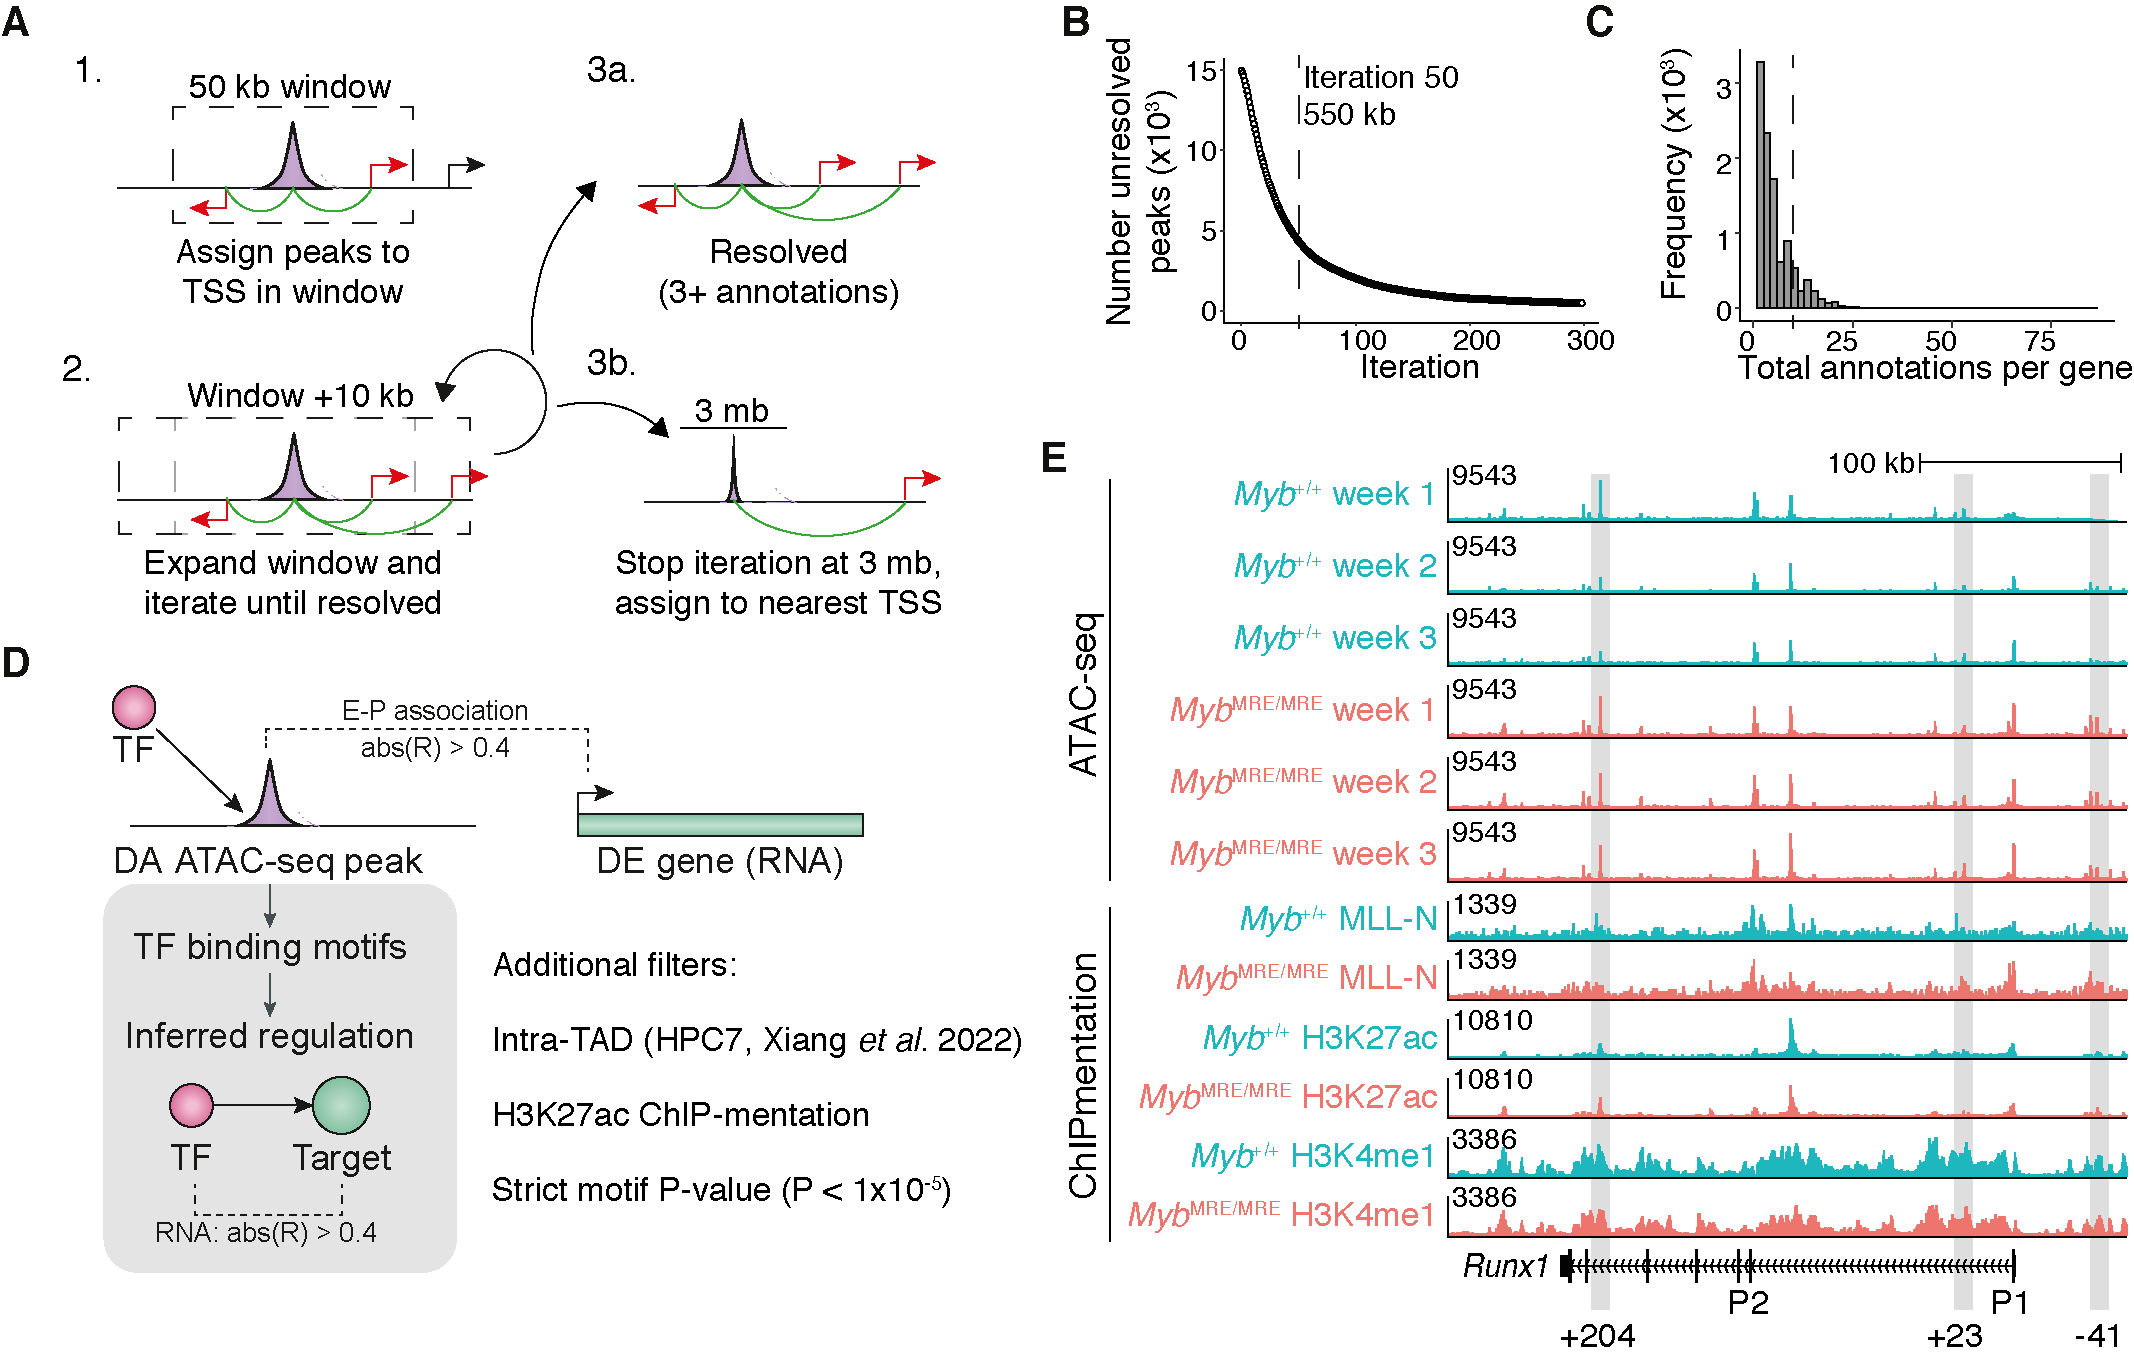
\includegraphics[width=\textwidth,height=\textheight,keepaspectratio]{figures/chapter5/ch5_gmp-grn.png}
    \caption[{Constructing a GRN model of MLL-AF9 GMP transformation.}]
    {\textbf{Constructing a GRN model of MLL-AF9 GMP transformation.}
    \textbf{(A)} Schematic of iterative peak calling approach. Peaks were assigned to any TSS in a 50 kb window, with further annotations added with incrementally larger windows (+10 kb per step). This iteration is performed for each peak, until resolved (3+ annotations per peak), or the window reaches 3 Mb. 
    \textbf{(B)} Number of unresolved peaks remaining at each step in the iterative peak calling method. Dashed line indicates the point of diminished returns, with majority of peaks resolved. 
    \textbf{(C)} Number of peaks annotated to each gene promoter using the iterative peak annotation approach. Dashed line indicates 10 annotations per gene.
    \textbf{(D)} Schematic outlining approach to generate the MLL-AF9 GMP GRN.
    \textbf{(E)} ATAC-seq and ChIPmentation tracks at \textit{Runx1}. GRN predicted differential enhancer elements highlighted in grey. ChIPmentation time points were combined into a single track for visualisation.
    }
    \label{fig:ch5_gmp-grn}
\end{figure}

In brief, differentially accessible enhancers were associated with all expressed promoters within a 50 kb window. To seed potential E-P interactions, I defined enhancers with three or more promoter links as sufficiently annotated (resolved). Unresolved enhancers underwent iterative annotations by increasing the annotation window by 10 kb each step, until resolved. For peaks with no annotations in a 3 Mb window, the nearest expressed promoter was annotated. Using this approach, the majority of peaks are resolved within a 550 kb window (Fig. \ref{fig:ch5_gmp-grn}B), and most genes had fewer than 10 enhancers annotated (Fig. \ref{fig:ch5_gmp-grn}C).

As in section \ref{ch3:grn} p.\pageref{ch3:grn}, to retain high confidence associations, E-P interactions were additionally filtered for greater than 0.4 correlation between enhancer ATAC-seq signal and promoter RNA expression (Fig. \ref{fig:ch5_gmp-grn}D). This method successfully allows annotating long-distance enhancers that span gene deserts, such as the \textit{Myc} +1.7 Mb super enhancer \citep{shi_role_2013} (Appendix \ref{fig:app_myc-annotation}), while limiting over-annotation in gene dense regions. E-P interactions are typically constrained by the boundaries of topologically associated domains (TADs, \cite{beagan_existence_2020}). Using published TAD data \citep{wilson_integrated_2016, xiang_integrative_2020} generated in the HPC7 cell line (ESC derived HPC model, \cite{pinto_do_o_expression_1998}), 76.2\% of E-P interactions assigned were found within TADs. In this analysis I reasoned that HPC7s were a reasonable model of GMPs, as TAD boundaries are thought to vary little between cell types \citep{beagan_existence_2020}. E-P interactions that spanned TAD boundaries were removed, as these likely represent erroneous annotations. Overall, this approach successfully annotates long-distance enhancers, such as the \textit{Myc} super enhancer, however without supplementary TAD data it over-calls distal enhancers.

To assemble the E-P interactions into a GRN model, as in section \ref{ch3:grn} p.\pageref{ch3:grn}, upstream regulators were inferred by the presence of TF binding motifs at enhancers and promoters (Fig. \ref{fig:ch5_gmp-grn}D). To improve confidence, motifs were filtered by P-value < \xten{1}{-6}, which still allows detection of the relatively short canonical Myb motif (5'-AACNG-3', \cite{ogata_solution_1994}). Regulatory interactions were filtered for correlation greater than 0.4 (or less than -0.4) between expression of the TF regulator and predicted target gene. The MLL-N ChIPmentation data was used to infer MLL-AF9 binding. This method is exemplified at the \textit{Runx1} locus, where the +23 and +204 enhancers were successfully identified, and are marked by H3K27ac and H3K4me1, as well as binding by MLL-AF9 (Fig. \ref{fig:ch5_gmp-grn}E). Together these data were integrated to establish an overall GRN model of the regulatory adaptations occurring after MLL-AF9 transduction. 

\section[Sub-networks can describe TFs driving expression modules]{\label{ch5:sub-grn}Sub-networks can describe TFs driving\\expression modules}

The GRN model is based on DEGs covering all time points, and includes gene expression data from both \mybwt{} and \mybmre{} samples. To determine the key drivers of this generalised GRN model, I calculated the most central nodes (Fig. \ref{fig:ch5_grn-vis}A). As the key driver of the leukaemia, MLL-AF9 is the most connected node. Interestingly, despite the impact of \textit{Myb} perturbation on MLL-AF9 leukaemia, Myb is not among the most central factors, at least within the overall network. While Myb is not the most connected, it may still regulate essential components of the leukaemic GRN. Similar to the MLL-AF4 GRN (Fig. \ref{fig:ch4_ma4-grn}B, p.\pageref{fig:ch4_ma4-grn}), Elf1, Egr1 and Mef2c are central factors in the MLL-AF9 GMP GRN, with Egr1 displaying the highest betweenness centrality (Fig. \ref{fig:ch5_grn-vis}A). 

\begin{figure}[htbp]
    \centering
    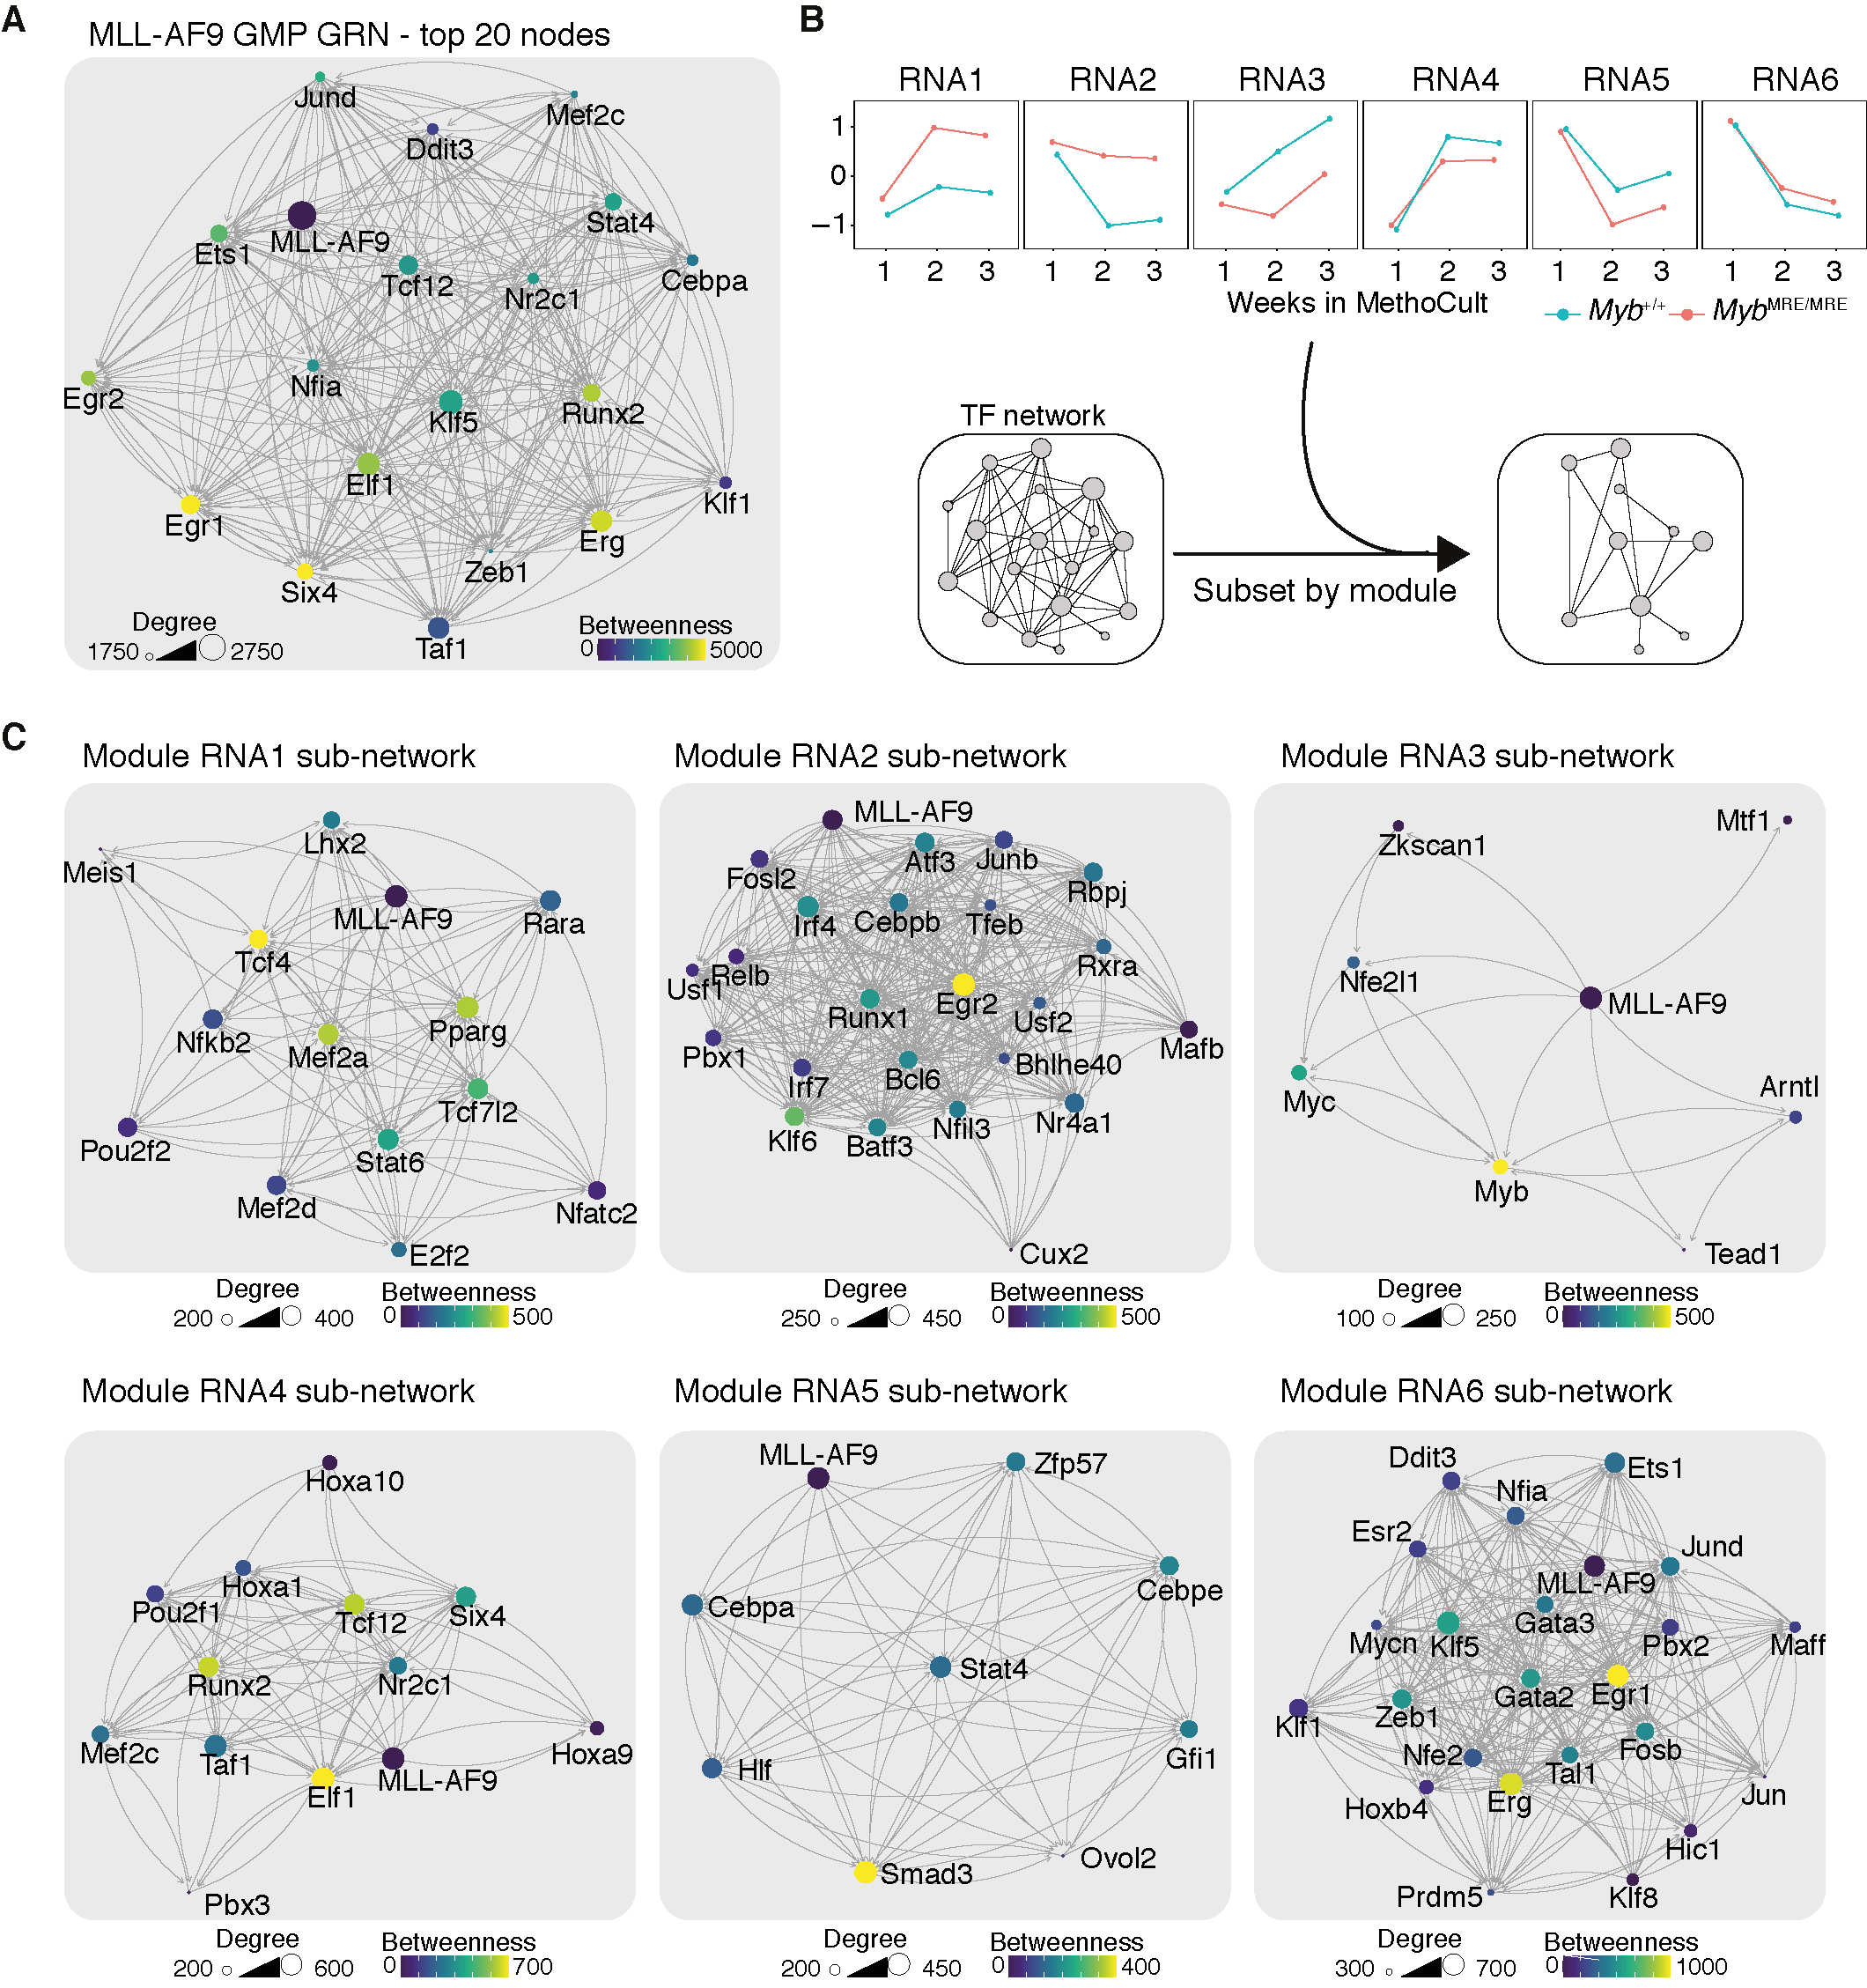
\includegraphics[width=\textwidth,height=\textheight,keepaspectratio]{figures/chapter5/ch5_grn-vis.png}
    \caption[{Generation and visualisation of MLL-AF9 GMP GRN sub-networks.}]
    {\textbf{Generation and visualisation of MLL-AF9 GMP GRN sub-networks.}
    \textbf{(A)} The top 20 genes of the MLL-AF9 GMP GRN by degree centrality.  
    \textbf{(B)} Illustration of sub-network generation, by filtering the overall MLL-AF9 GMP GRN by RNA-seq module genes (RNA1-6), derived in Fig. \ref{fig:ch5_profiles}C-D. 
    \textbf{(C)} Sub-networks based on RNA modules, generated as in B. Sub-networks show all hub-node TFs expressed in each module. 
    For all network visualisations, size represents degree centrality, while colour represents betweenness centrality. Lines indicate predicted interaction from protein to gene locus, with arrowheads pointing downstream. 
    }
    \label{fig:ch5_grn-vis}
\end{figure}

As the GRN model describes both \mybwt{} and \mybmre{} gene expression, it is important to then decode the network to query specific questions. The RNA gene expression modules (RNA1-6, Fig. \ref{fig:ch5_profiles}C-D) were used to decode the network by creating GRN sub-networks based on module genes, followed by recalculation of centrality measures (Fig. \ref{fig:ch5_grn-vis}B). Module RNA3, encompassing TFs that display much higher expression in \mybwt{} samples over \mybmre{}, contains both Myb and Myc, both of which display high degree and betweenness centrality (Fig. \ref{fig:ch5_grn-vis}C). This aligns with the critical function of both these TFs in leukaemia, and suggests that they may be driving the \mybmre{} phenotype. RNA4 genes show slightly increased expression in \mybwt{} over \mybmre{}, and the TFs Runx2 and Elf1 show the highest degree and betweenness centrality within its sub-network. This module also contains Hoxa1, Hoxa9, and Hoxa10, suggesting the \textit{Hoxa} cluster overall is repressed in \mybmre{} samples. This analysis confirms that Myb is an important driver of transcription, most specifically within the RNA3 sub-network, and is associated with significant downregulation in the \mybmre{} genotype. Similarly, TFs such as Runx2 and Elf1, as well as multiple hox genes, may drive lesser downregulation in the \mybmre{} genotype, through the RNA4 sub-network.


\section{\label{ch5:myc}\textit{Myc} upregulation occurs at week 3, after activation of multiple predicted regulators}

As discussed in section \ref{ch4:tf-cointeraction} p.\pageref{ch4:tf-cointeraction}, \textit{Myc} is a critical target in \textit{MLL}r leukaemias that we found to be activated synergistically by both Runx1 and Myb (Fig. \ref{fig:ch4_tf-coop-kd}, p.\pageref{fig:ch4_tf-coop-kd}, \cite{harman_kmt2a-aff1_2021}). The clustering and sub-network analysis (section \ref{ch5:sub-grn}) placed \textit{Myc} in module RNA3. However, while \textit{Myc} does show slightly decreased expression in \mybmre{} samples, it is not affected to the same extent as other RNA3 members, such as \textit{Myb} (Fig. \ref{fig:ch5_myc-regulation}A). Interestingly, while the majority of transcriptional changes in this system occur between W1 and W2 (Fig. \ref{fig:ch5_profiles}B-D), \textit{Myc} expression is primarily upregulated from W2 to W3 (Fig. \ref{fig:ch5_myc-regulation}A). 

%\vspace*{0.5in}
\begin{figure}[!t]
    \centering
    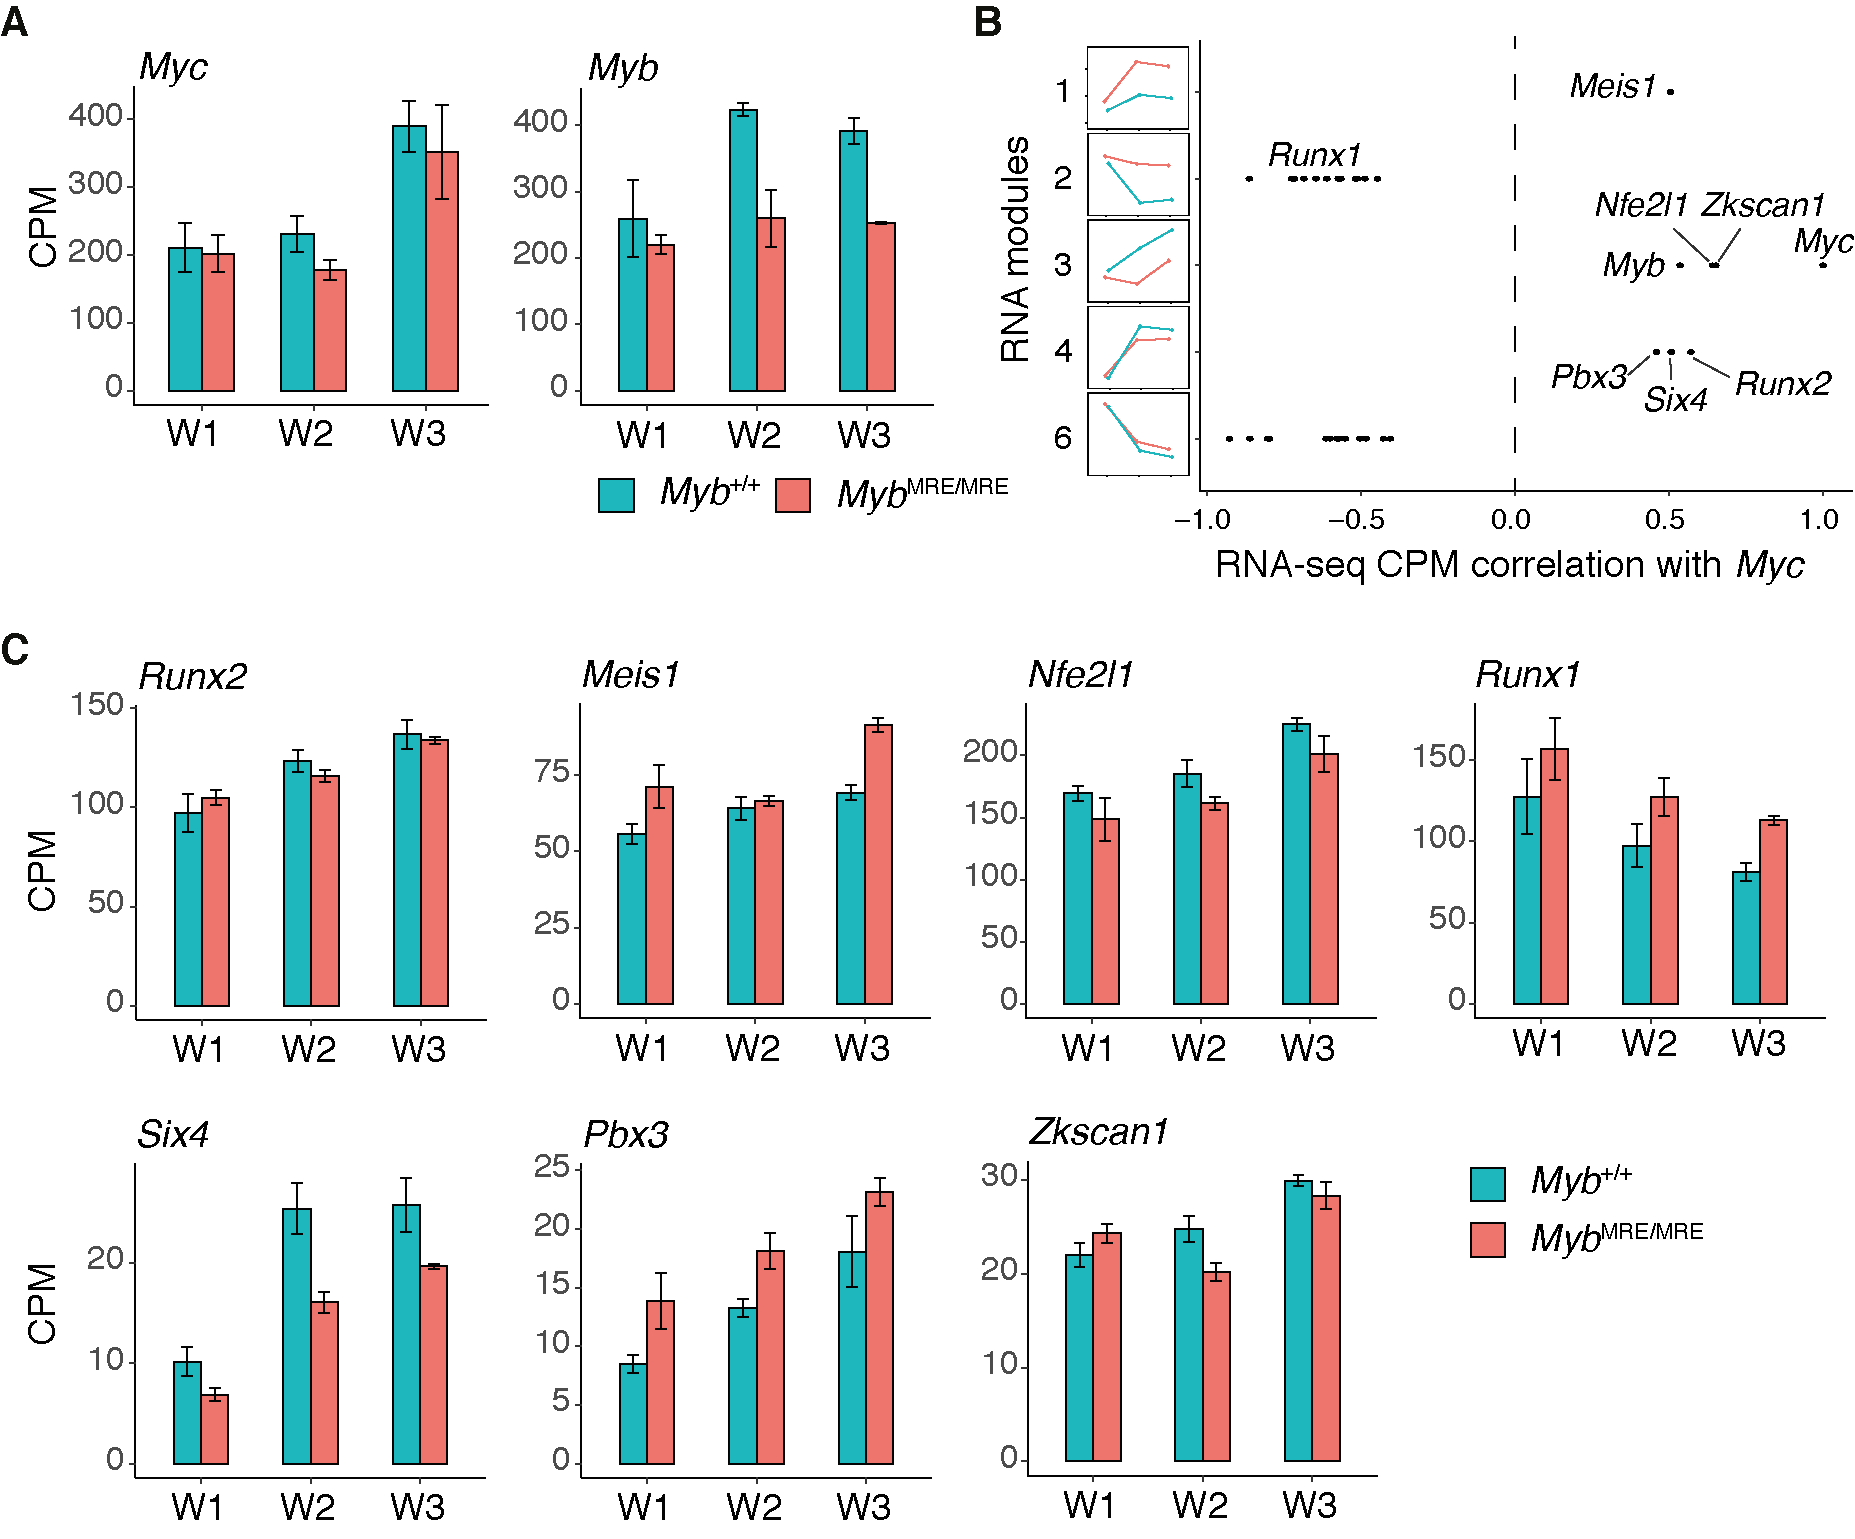
\includegraphics[width=\textwidth,height=\textheight,keepaspectratio]{figures/chapter5/ch5_myc-regulation.png}
    \caption[{\textit{Myc} is not fully expressed until week 3, potentially through additional TF regulators.}]
    {\textbf{\textit{Myc} is not fully expressed until week 3, potentially through additional TF regulators.}
    \textbf{(A)} Gene expression (CPM) for \textit{Myc} and \textit{Myb}. Error bars represent standard error of the mean; \textit{n} = 3. 
    \textbf{(B)} RNA correlation between \textit{Myc} and predicted \textit{Myc} regulators, stratified by RNA-seq expression modules. Illustrative representation of modules shown along the y-axis. 
    \textbf{(C)} Gene expression (CPM) for predicted \textit{Myc} regulators positively correlated with \textit{Myc} expression. Error bars represent standard error of the mean; \textit{n} = 3.
    }
    \label{fig:ch5_myc-regulation}
\end{figure}

%\clearpage

To understand this delayed activation of \textit{Myc}, I explored its predicted upstream regulators (Fig. \ref{fig:ch5_myc-regulation}B-C). \textit{Myb} expression is reasonably correlated with \textit{Myc}, though \textit{Myb} perturbation in \mybmre{} does not have a strong effect on \textit{Myc} regulation. \textit{Runx1} is instead anti-correlated with \textit{Myc}, which disagrees with the MLL-AF4 GRN model (Fig. \ref{fig:ch4_tf-coop-kd}, p.\pageref{fig:ch4_tf-coop-kd}), and could suggest that Runx1 activity differs in the MLL-AF9 GMP context. In fact, \textit{Runx1} deletion is known to impair lymphopoiesis but increase myeloid cell expansion \citep{growney_loss_2005, ichikawa_aml-1_2004}, and has been proposed to repress \textit{Myc} in AML via a FOXC3/RUNX1/HDAC1/TLE3 repressor complex \citep{simeoni_enhancer_2021}. Multiple predicted regulators are positively correlated with \textit{Myc} expression, including \textit{Runx2}, \textit{Meis1}, and \textit{Nfe2l1} (Fig. \ref{fig:ch5_myc-regulation}B-C). However, none of these TFs strongly correlate with \textit{Myc}, and they are not upregulated primarily from W2 to W3, but instead generally show continual upregulation from W1 to W3. It is possible that multiple TFs must first be activated and could be required to cooperate before \textit{Myc} upregulation occurs, contributing to this delayed gene expression response.

\section[Myb and MLL-AF9 are predicted to co-interact with a range of TFs to drive leukaemogenesis]{\label{ch5:co-interact}Myb and MLL-AF9 are predicted to\\co-interact with a range of TFs to drive\\leukaemogenesis}

To investigate how Myb and MLL-AF9 may cooperate with other TFs, I applied the same analytical approach as in section \ref{ch3:co-interaction}, p.\pageref{ch3:co-interaction} (methods section \ref{ch2:coint-methods}, p.\pageref{ch2:coint-methods}) to identify probable cases of TF co-interaction. As previously, I performed Fisher's exact tests for predicted targets across all TF pairs, and clustered odds ratio scores describing the likelihood that TF pairs co-interact more frequently than random. This resulted in six co-interaction clusters representing groups of TFs that may cooperate (CoInt 1-6, Fig. \ref{fig:ch5_co-interaction}A). CoInt-1 contains Hox TFs and CoInt-4 contains Gfi1 and Meis1, and both clusters are enriched for general haematopoiesis and differentiation terms (Fig. \ref{fig:ch5_co-interaction}A-B). CoInt-2 contains Myb, Runx1, and MLL-AF9 and is enriched for differentiation processes in both myeloid and lymphoid lineages (Fig. \ref{fig:ch5_co-interaction}A-B). CoInt-5 contains several central factors, including Elf1 and Runx2, but shows little pathway enrichment, while CoInt-6 includes Smad3 and is correspondingly enriched for BMP signalling (Fig. \ref{fig:ch5_co-interaction}A-B).

%\vspace*{0.7in}
\begin{figure}[!t]
    \centering
    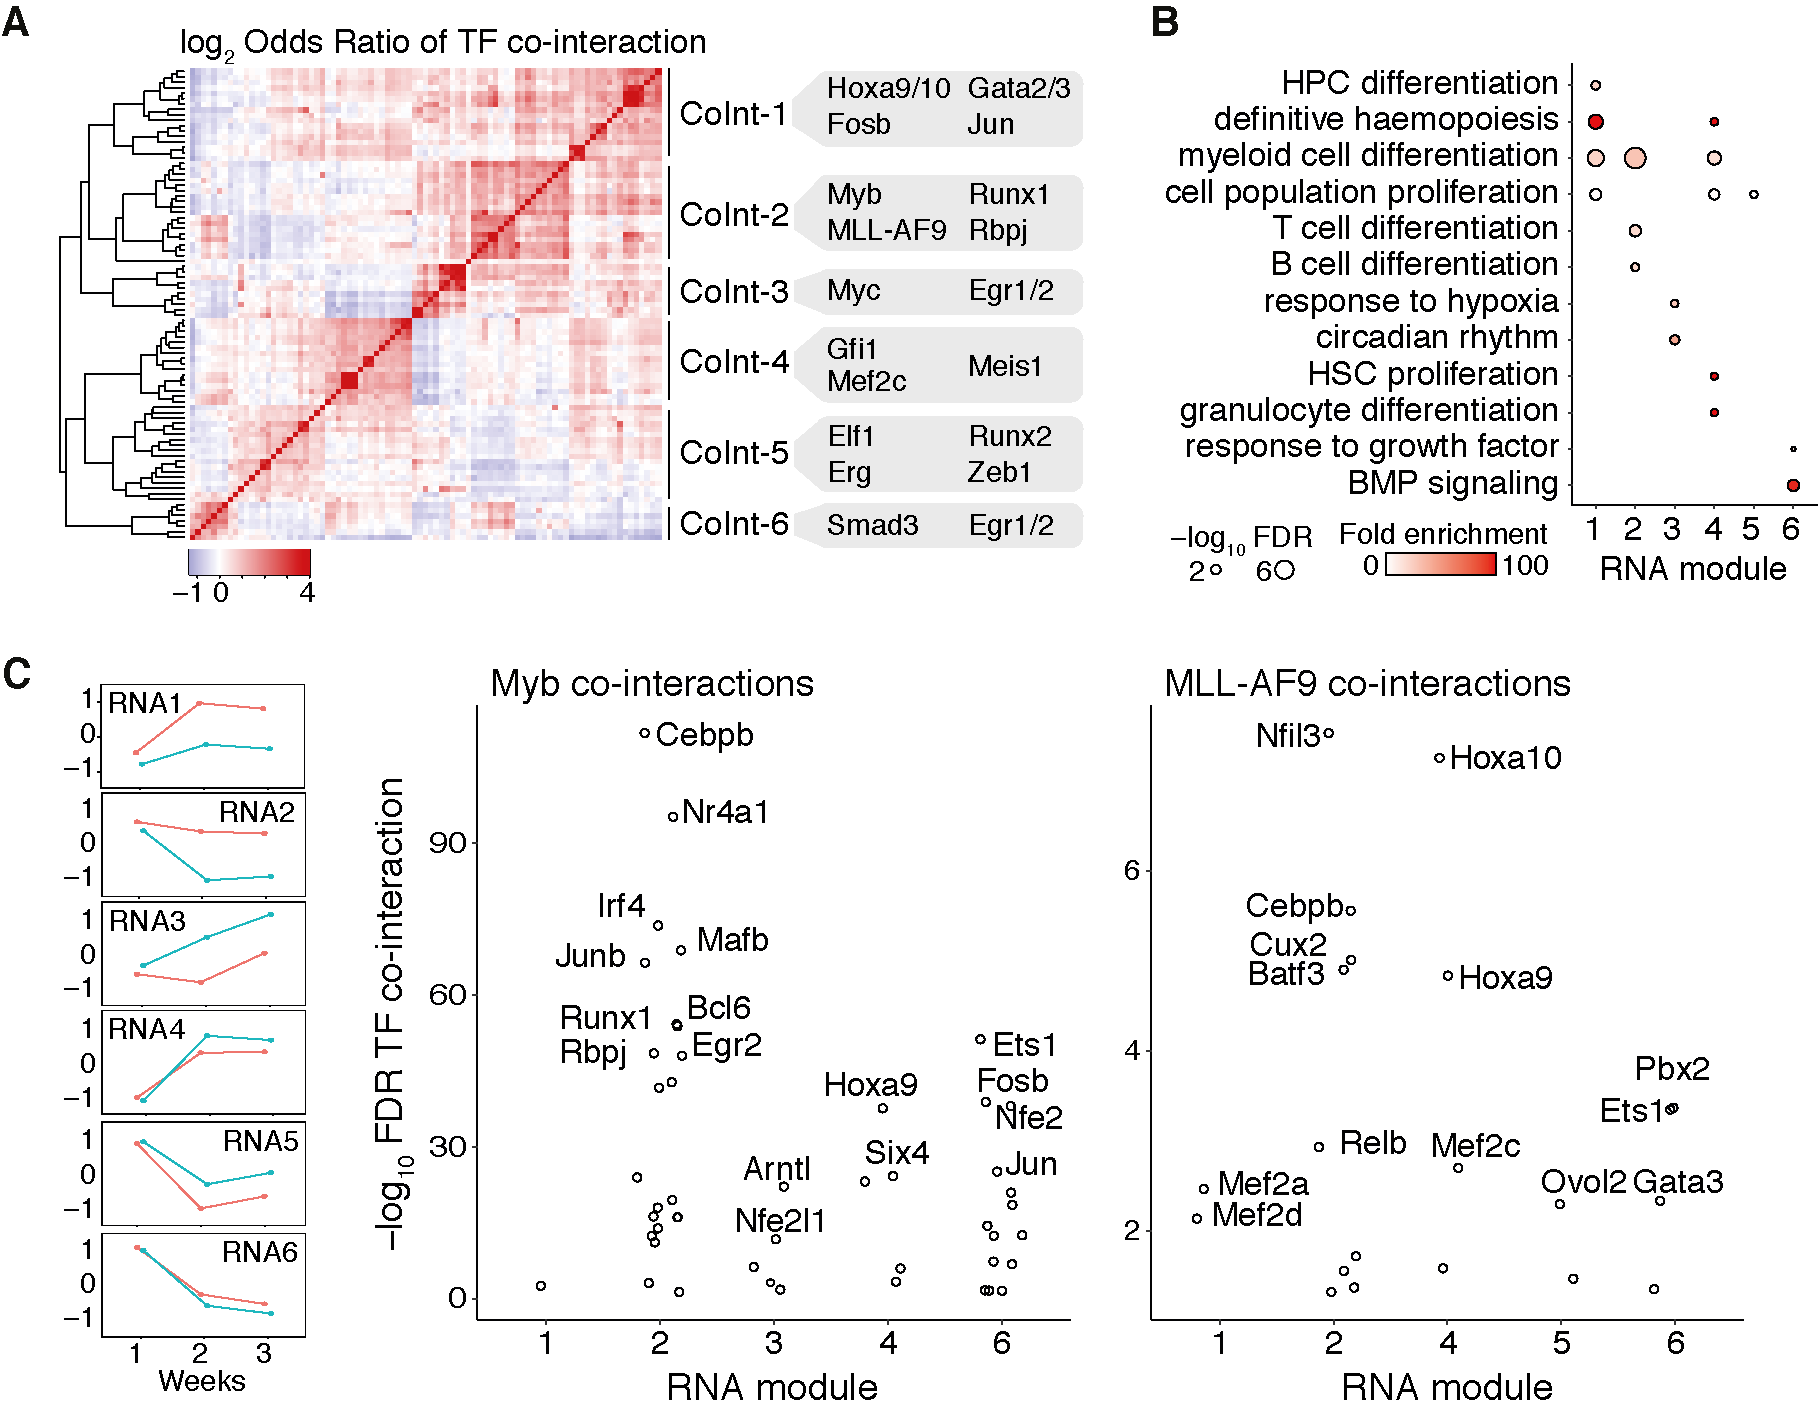
\includegraphics[width=\textwidth,height=\textheight,keepaspectratio]{figures/chapter5/ch5_co-interaction.png}
    \caption[{TF co-interaction drives differentiation, growth, and signalling pathways.}]
    {\textbf{TF co-interaction differentiation, growth, and signalling pathways.}
    \textbf{(A)} Hierarchical clustered heatmap of Fisher's exact test odds ratios comparing the overlap of TF-targets between pairs of TFs. Benjamini and Hochberg correction of P values was performed, and TFs not significant for any interaction were excluded. Clusters describe sets of TFs that commonly act at the same loci, suggesting cooperative regulation. Example TFs present in each cluster are given. 
    \textbf{(B)} GO biological process enrichment for clusters CoInt 1-6, as in A. Only significant data points shown (P $\leq$ 0.05). 
    \textbf{(C)} Significance of TF co-interactions with Myb or MLL-AF9, as calculated in A, stratified by RNA modules (RNA1-6). RNA-seq expression modules shown on left for reference. 
    }
    \label{fig:ch5_co-interaction}
\end{figure}
%\clearpage

As Myb and MLL-AF9 are key factors in this system, I focused the analysis to predict their co-interaction partners (Fig. \ref{fig:ch5_co-interaction}C). MLL-AF9 has widespread binding and regulates many targets, but still shows significant co-interaction with specific TFs. These include Hoxa9 and Hoxa10, Nfil3, Cebpb, and Cux2. For Myb co-interactions, among RNA3 module genes Arntl and Nfe2l1 are both predicted to co-interact with Myb. Arntl (known as Bmal1) is a core circadian rhythm TF that has been shown to be important \textit{MLL}r AML progression \citep{puram_core_2016}. It is possible that Arntl cooperates with Myb to affect downstream targets, as part of the circadian rhythm. The most significant Myb co-interactors are expressed in RNA2, which shows an opposite expression pattern to Myb, and includes Cebpb, Nr4a1, and Irf4. Interestingly, the well-known MLL-FP target \textit{Hoxa9} \citep{milne_multiple_2010} significantly co-interacts with both Myb and MLL-AF9. Despite a differing expression pattern, Runx1 still significantly co-interacts with Myb, suggesting that while Runx1 may have different activity in AML it could still cooperate with Myb. This preliminary analysis begins to explore potential TF cooperation that may drive key processes. Further investigation is necessary to establish key regulatory motifs.

\section{\label{ch5:myb-runx1}Myb and Runx1 may cooperate to drive expression of key regulatory hubs.}

As we have previously established, MYB and RUNX1 function cooperatively in the regulation of \textit{Myc} in MLL-AF4 ALL (section \ref{ch4:tf-cointeraction}, p.\pageref{ch4:tf-cointeraction}), and Myb appears to significantly co-interact with Runx1 in the MLL-AF9 GMP GRN (Fig. \ref{fig:ch5_co-interaction}C). I therefore explored potential cooperative regulation driven by these TFs. While Runx1 shows a different expression pattern to Myb (RNA2 and RNA3 respectively), and may act repressively in AML \citep{simeoni_enhancer_2021}, Runx1 is expressed throughout the time course and as such could still cooperate with Myb. To determine whether these TFs regulate similar targets I compared their regulatory logic. Both Myb and Runx1 preferentially target genes in expression modules RNA2, RNA3, RNA4 and RNA6, with few targets in RNA1 and RNA5 (Fig. \ref{fig:ch5_myb-runx1}A). In comparison, MLL-AF9 binds a high proportion of genes across all RNA modules. In addition to regulating similar gene classes, 48.5\% of Myb targeted accessible elements are also predicted targets of Runx1 (Fig. \ref{fig:ch5_myb-runx1}B). This shows that alongside a high significance of co-interaction, Myb and Runx1 show similar regulatory patterns across expression modules and a high rate of overlap across enhancers and promoters.

\begin{figure}[htbp]
    \centering
    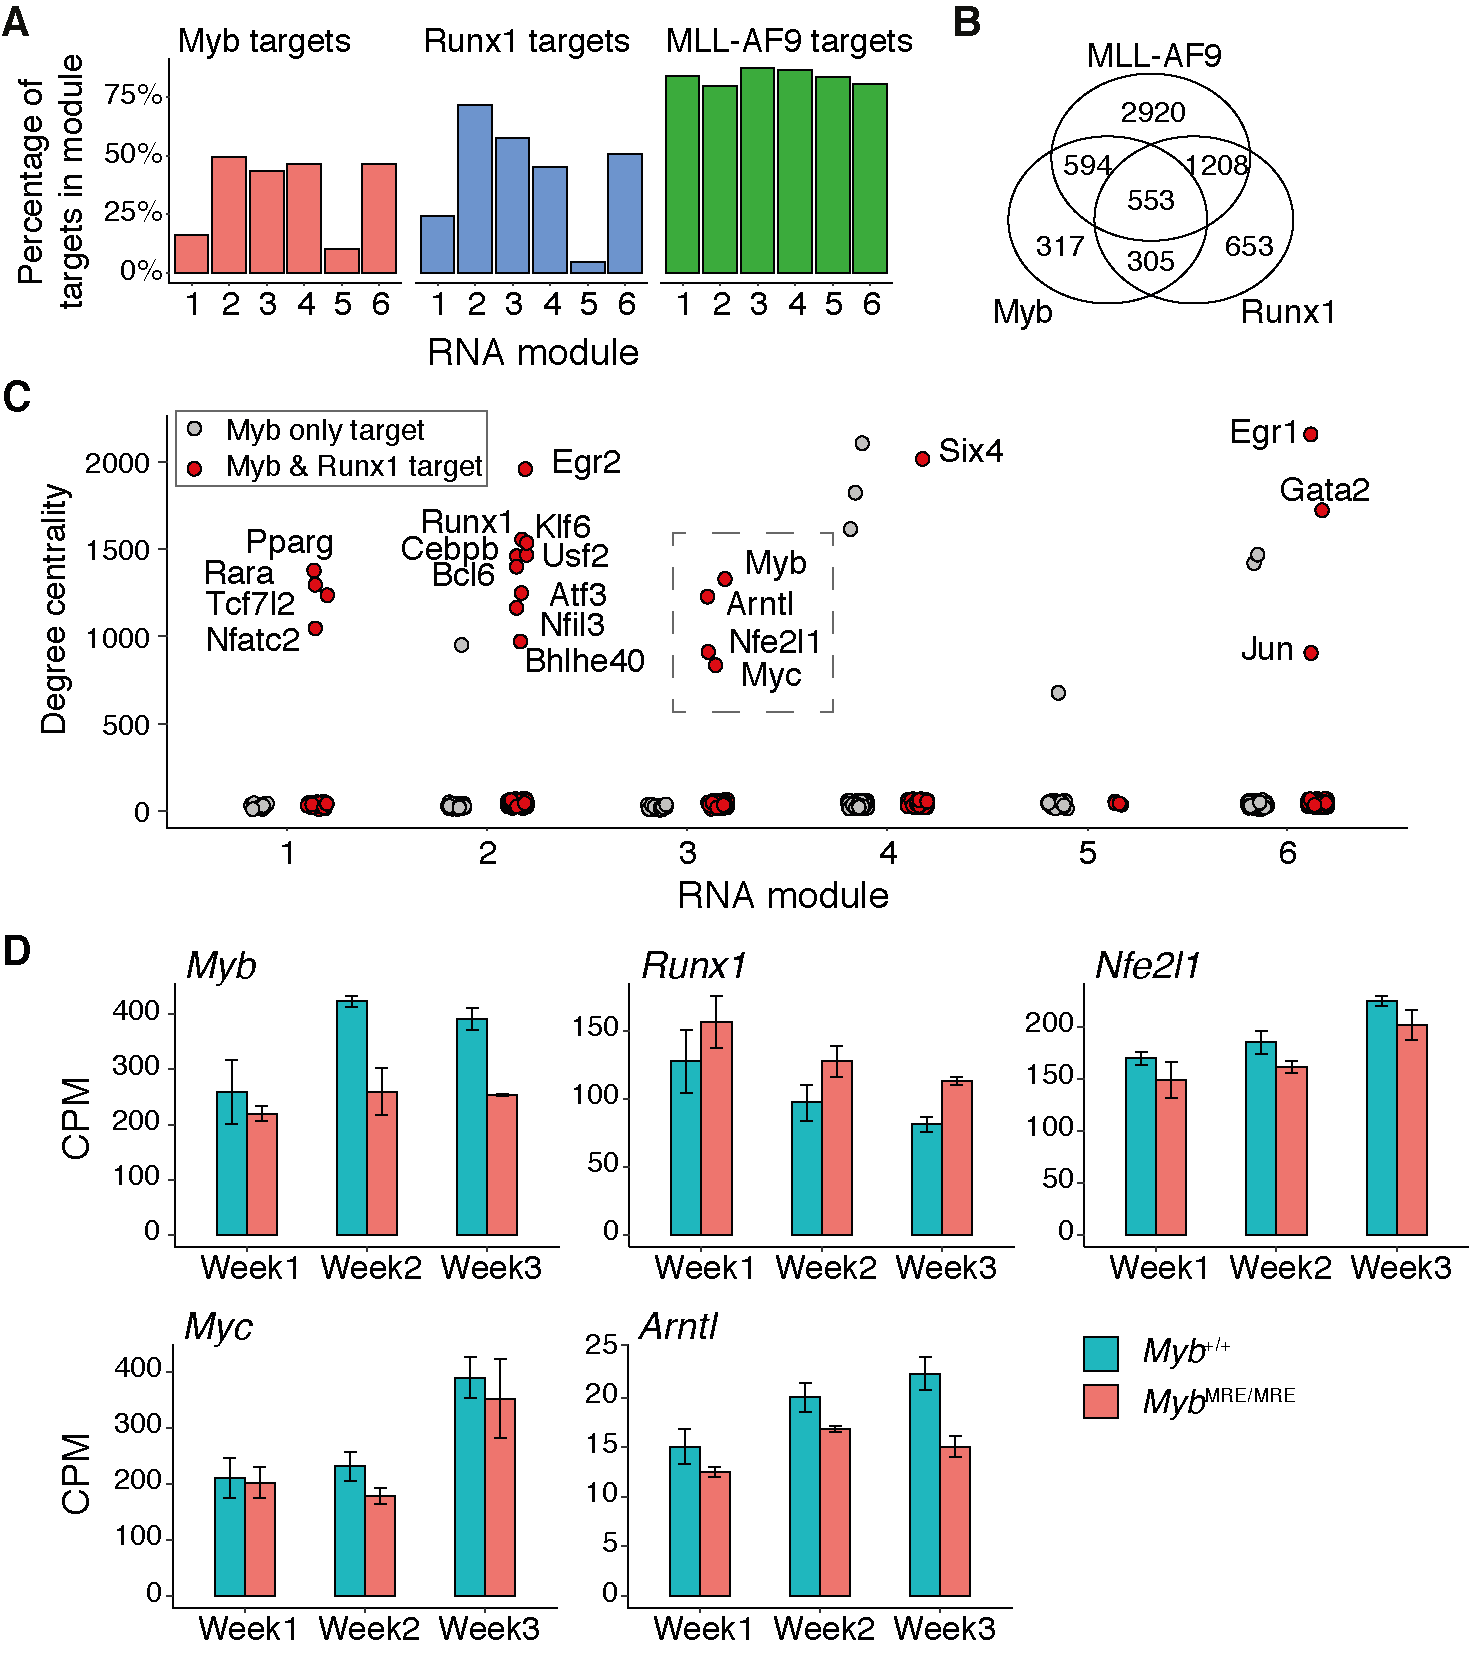
\includegraphics[width=\textwidth,height=\textheight,keepaspectratio]{figures/chapter5/ch5_myb-runx1.png}
    \caption[{Myb and Runx1 co-interact at multiple loci.}]
    {\textbf{Myb and Runx1 co-interact at multiple loci.}
    \textbf{(A)} Proportion of genes within each RNA-seq expression module with predicted targeting by Myb, Runx1, or MLL-AF9. 
    \textbf{(B)} Overlap of nodes between predicted Myb, Runx1, and MLL-AF9 target accessible elements. 
    \textbf{(C)} Stratification of degree centrality (MLL-AF9 GMP GRN) by RNA-seq expression modules. Data points coloured by whether they are targeted by Myb, or Myb and Runx1. Dashed box highlights RNA3 genes with predicted regulation from both Runx1 and Myb.
    \textbf{(D)} CPM expression for \textit{Runx1} and RNA3 module genes targeted by both Myb and Runx1. Error bars represent standard error of the mean; \textit{n} = 3. 
    }
    \label{fig:ch5_myb-runx1}
\end{figure}

As TFs are important regulators of \textit{MLL}r leukaemias, I explored whether Runx1 and Myb co-regulate GRN regulatory hubs (Fig. \ref{fig:ch5_myb-runx1}C). Despite Runx1 and Myb co-interacting at 48.5\% of Myb-targeted elements, of predicted Myb-regulated TFs (28 genes) 75\% (21 genes) are also predicted to be regulated by Runx1. Focusing specifically on RNA3 genes, which displayed the greatest difference between \mybwt{} and \mybmre{} genotypes, Myb and Runx1 appear to co-regulate \textit{Myc}, \textit{Nfe2l1}, and \textit{Arntl} (Fig. \ref{fig:ch5_myb-runx1}D). As \textit{Runx1} expression decreases over time while these targets are upregulated, it might be expected that Runx1 plays an inconsequential or repressive role at these sites. However, it is possible that Runx1 behaves differently at sites also bound by Myb, or that Runx1 supports Myb activity. It has been reported that Runx1 acts synergistically with Myb in neutrophil myelopoiesis in zebrafish \citep{huang_runx1_2021} and so it remains possible, though as yet unexplored, that Runx1 positively regulates these targets along with Myb.


\section{\label{ch5:myb-runx1-essential}Myb perturbation may cooperate with Runx1 to impact leukaemogenesis and dysregulate essential targets.}

It is possible that Runx1 promotes greater Myb regulatory potential. While we do not have \textit{Runx1} perturbation data in this system to investigate this possibility, we can examine whether Myb:Runx1 co-regulated genes are more sensitive to \textit{Myb} suppression. I performed a differential comparison between \mybwt{} and \mybmre{} samples. In this comparison, I modelled time (Weeks 1-3) as a blocking factor, such that variation due to time in culture is removed (methods section \ref{ch2:rna-analysis}, p.\pageref{ch2:rna-analysis}). DEGs from this test therefore represented general differences in \textit{Myb} genotype, rather than week-specific effects. This resulted in 1031 differentially expressed GRN nodes (Fig. \ref{fig:ch5_myb-runx1-wt-mre}A). Downregulated genes in this comparison (lower expression in \mybmre{}) were primarily in expression modules RNA3, RNA4 and RNA5, whereas RNA1 and RNA2 contained upregulated genes. To interrogate positive Myb activity in the context of Runx1 predicted regulation, I explored logFC distributions in RNA3-5, and found that at Myb:Runx1 co-regulated targets, gene expression was reduced to a greater extent in \mybmre{} than genes predicted to be regulated by Myb without Runx1, though the effect was subtle (Fig. \ref{fig:ch5_myb-runx1-wt-mre}B). The difference in logFC was greater at RNA4-5 than RNA3. This effect was also seen in RNA1 and RNA2, where Myb:Runx1 predicted co-regulation confers greater upregulation. This analysis suggests that Myb may enact stronger regulation in the context of Runx1, though whether this is through direct cooperation with Runx1 needs to be explored.

\begin{figure}[!t]
    \centering
    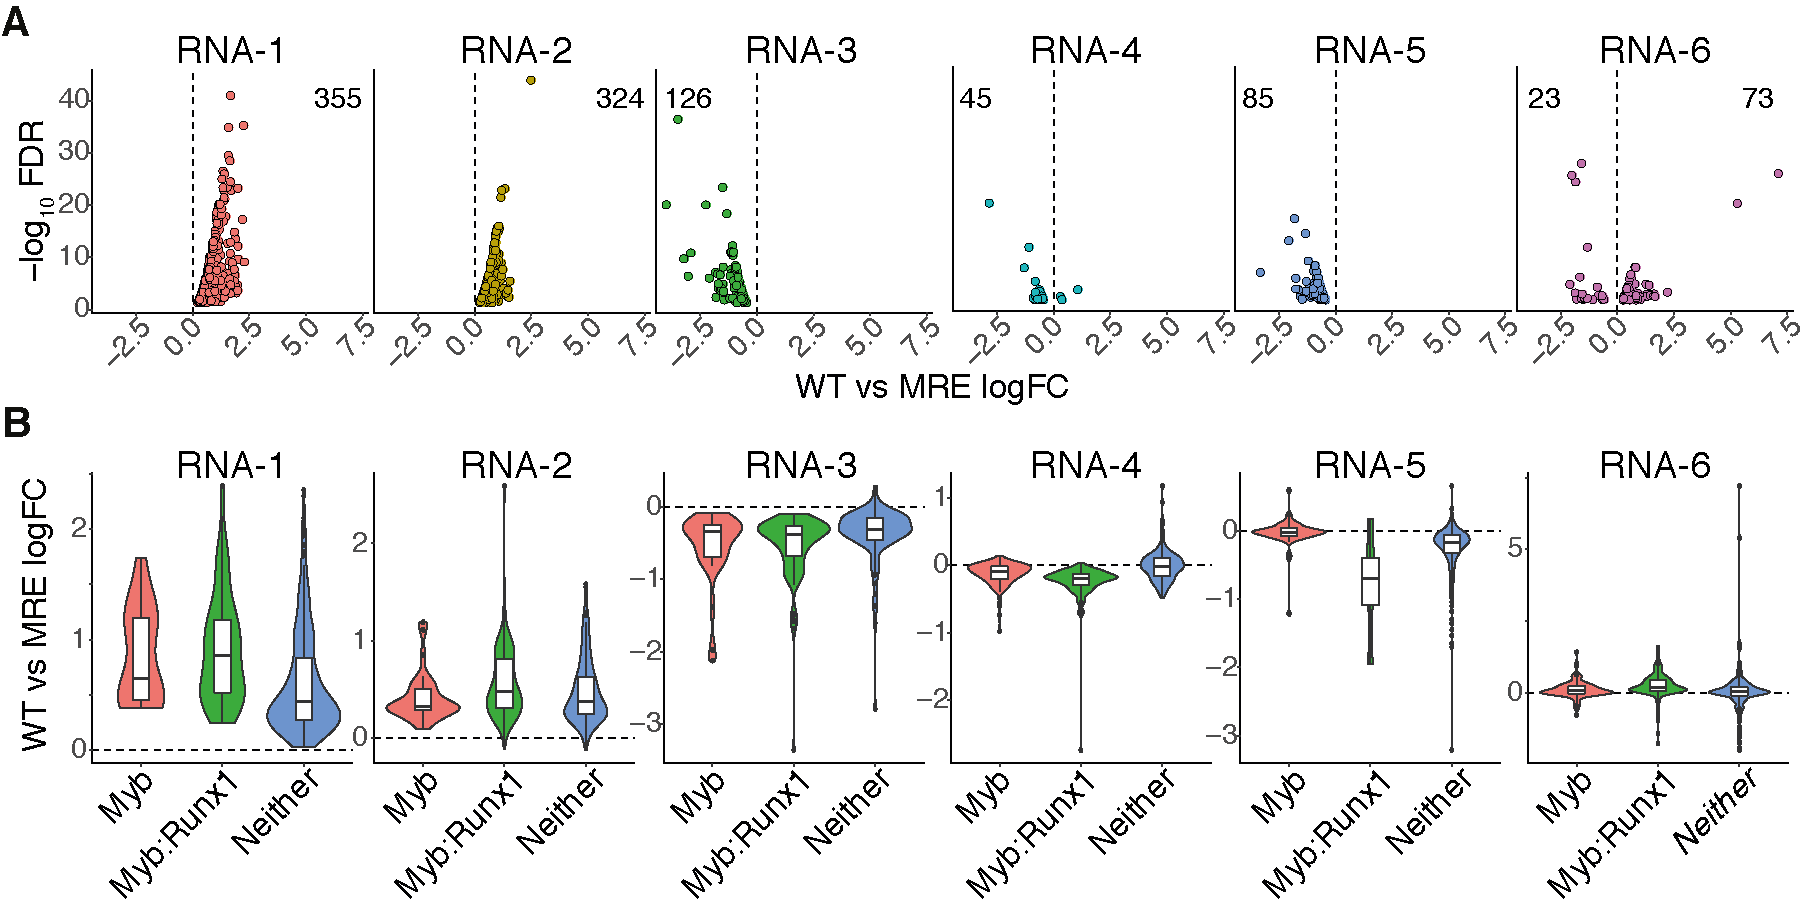
\includegraphics[width=\textwidth,height=\textheight,keepaspectratio]{figures/chapter5/ch5_myb-runx1-wt-mre.png}
    \caption[{Myb and Myb:Runx1 target genes are more sensitive to \textit{Myb} perturbation by the \mybmre{} circuit.}]
    {\textbf{Myb and Myb:Runx1 target genes are more sensitive to \textit{Myb} perturbation by the \mybmre{} circuit.}
    \textbf{(A)} Relationship between -log\textsubscript{10} FDR and logFC (comparing \mybwt{} and \mybmre{}; positive logFC means higher expression in \mybmre{}), in the MLL-AF9 GMP RNA-seq data. Results are stratified and coloured by RNA-seq expression modules. 
    \textbf{(B)} Violin and boxplot summary of logFC values (comparing \mybwt{} and \mybmre{}), stratified by RNA-seq expression modules. Data coloured by whether genes are targeted by Myb only, or Runx1 and Myb, or neither. 
    }
    \label{fig:ch5_myb-runx1-wt-mre}
\end{figure}

\begin{figure}[!t]
    \centering
    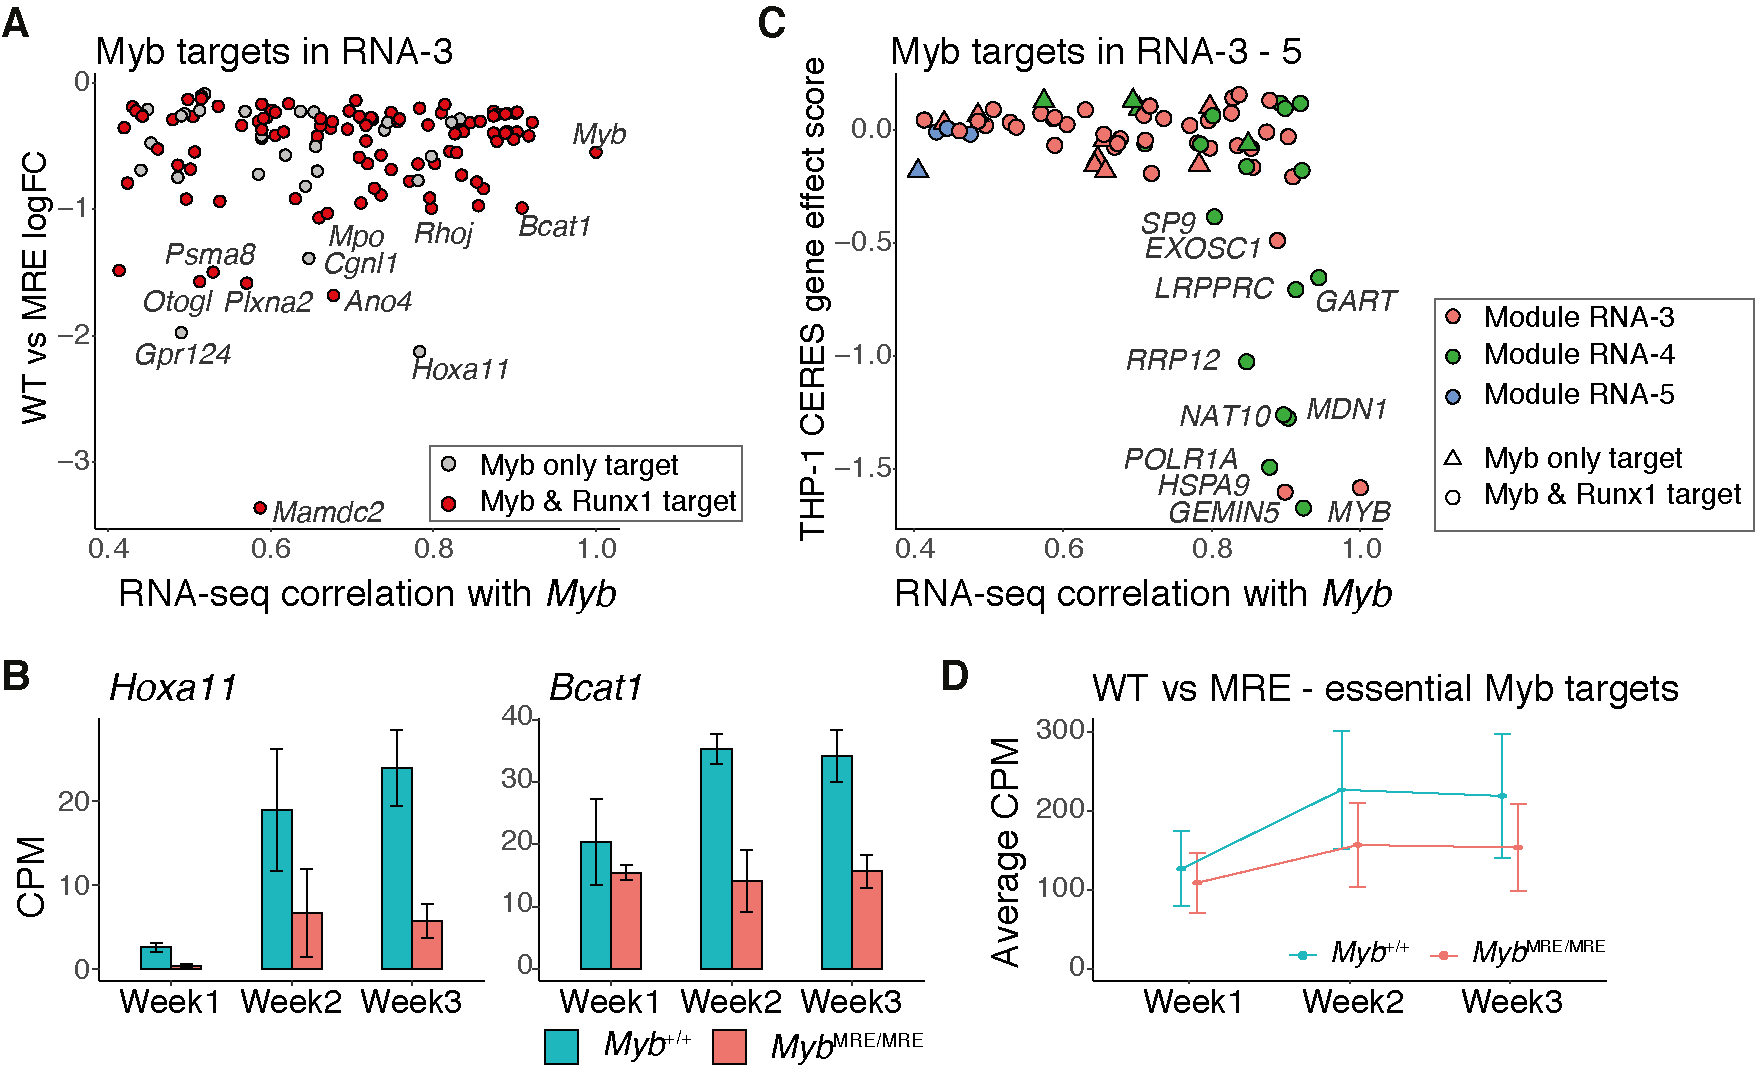
\includegraphics[width=\textwidth,height=\textheight,keepaspectratio]{figures/chapter5/ch5_essential-targets.png}
    \caption[{\textit{Myb} is highly correlated with essential genes impacted by the \mybmre{} circuit.}]
    {\textbf{\textit{Myb} is highly correlated with essential genes impacted by the \mybmre{} circuit.}
    \textbf{(A)} Association between RNA-seq logFC values comparing \mybwt{} and \mybmre{} and expression correlation with \textit{Myb}. Data points shown are predicted Myb targets with FDR < 0.05 when comparing \mybwt{} and \mybmre{}, and are coloured by whether genes are targeted by Myb only, or Runx1 and Myb. 
    \textbf{(B)} Gene expression (CPM) for \textit{Hoxa11} and \textit{Bcat1}, as highlighted in A. Error bars represent standard error of the mean; \textit{n} = 3. 
    \textbf{(C)} Association between expression correlation with \textit{Myb}, and THP-1 gene essentiality scores (CERES), where lower CERES scores indicate greater essentiality. Mouse genes were  mapped to human gene symbols. Data points shown are predicted Myb targets in modules RNA3-5, with FDR < 0.05 when comparing \mybwt{} and \mybmre{}. Genes are considered essential below CERES score -0.5. Colour represents gene expression module, while shape represents targeting by Myb only, or Runx1 and Myb. 
    \textbf{(D)} Average gene expression (CPM) plots for all \textit{Myb} correlated and essential genes highlighted in C. Data points represent mean CPM across all genes, and bars represent standard error of the mean.  
    }
    \label{fig:ch5_essential-targets}
\end{figure}

To focus on the activity of Myb, I used the RNA-seq module RNA3, which shows the greatest difference in expression with \textit{Myb} perturbation (\mybmre{}). I took predicted Myb targets in the RNA3 expression module and stratified these by logFC (comparing \mybwt{} and \mybmre{}) and gene expression correlation with \textit{Myb} (Fig. \ref{fig:ch5_essential-targets}A). Two genes highly downregulated in \mybmre{}, and highly correlated with \textit{Myb} expression (R > 0.7), were Hoxa11 and Bcat1. \textit{Hoxa11} is predicted to be regulated by Myb and not Runx1, is downregulated in \mybmre{} samples, and is highly correlated with \textit{Myb} expression (Fig. \ref{fig:ch5_essential-targets}A-B). \textit{Bcat1}, which is predicted to be co-regulated by both Myb and Runx1, is moderately downregulated in \mybmre{} samples and has very high \textit{Myb} expression correlation (R > 0.9). A previous study has found \textit{Bcat1} to be overexpressed in AML patients and associated with poor prognosis, as well as to drive DNA hypermethylation similar to IDH\textsuperscript{mut} AML \citep{raffel_bcat1_2017}. In contrast to the \mybwt{} samples, in \mybmre{} \textit{Bcat1} expression remains the same across all weeks (Fig. \ref{fig:ch5_essential-targets}B), suggesting that MLL-AF9 alone does not drive expression over MethoCult expansion and that this overexpression is dependent on Myb. This preliminary exploration begins to identify potential mechanisms by which Myb promotes leukaemogenesis, and in the case of \textit{Bcat1} may indicate a mechanism independent of MLL-AF9.

While the \mybmre{} genotype accompanies defects in leukaemic growth \citep{lau_role_2022}, it is as yet unclear which Myb interactions are critical for leukaemogenesis. To address this question, I estimated the importance of genes for leukaemogenesis with CRISPR essentiality data in THP-1 cells (MLL-AF9 AML cell line) from DepMap (22Q2 dataset, \cite{meyers_computational_2017, doench_optimized_2016}), using data for human orthologues of mouse gene targets. I compared CRISPR essentiality scores against \textit{Myb} gene expression correlation at Myb target genes (Fig. \ref{fig:ch5_essential-targets}C). This analysis was performed on genes downregulated in \mybmre{} samples in modules RNA3-5. Strikingly, the most essential Myb target genes were all highly correlated with \textit{Myb} expression, while low or moderately correlated targets displayed no essentiality (Fig. \ref{fig:ch5_essential-targets}C). Further, all of these essential genes were also predicted to be regulated by Runx1. This suggests that these essential genes are strongly associated with Myb expression levels, and may be supported by Runx1 activity. These genes are all expressed at a much lower level in \mybmre{} samples over \mybwt{} (Fig. \ref{fig:ch5_essential-targets}D). This analysis provides a mechanism by which \textit{Myb} perturbation impairs leukaemogenesis, and highlights the association of Myb activity with essential downstream targets. It remains a question for future study as to whether Runx1 plays a role at these targets.

\clearpage
\section{Conclusions and discussion}

In this chapter, I have used a system established by I. Lau (Milne lab, \cite{lau_role_2022}) to transfect mouse GMPs with an \textit{MLL-AF9} expressing construct, and track gene expression changes over three weeks in culture. In doing so, I have established a set of experiments profiling gene expression, chromatin accessibility, and epigenetic modifications that monitor regulatory adaptations of \textit{MLL-AF9} expression. By including \mybmre{} mouse models, these datasets also track how these cells adapt to \textit{MLL-AF9} expression in the context of \textit{Myb} perturbation. I have integrated this data together into an overall GRN model (section \ref{ch5:grn}), that can be decoded to ask specific questions using gene expression modules (section \ref{ch5:sub-grn}). This data, while not yet fully explored, gives insight into how the wider regulatory network adapts to \textit{MLL-AF9} expression, and how Myb activity affects leukaemogenesis.

In exploring RNA-seq and ATAC-seq data, it was found that the W1 time point was significantly different from W2 and W3, in both transcription and chromatin accessibility (section \ref{ch5:profiles}, Fig. \ref{fig:ch5_profiles}). Interestingly, while W2 and W3 samples showed similar expression and accessibility profiles, it is at these time points that \mybwt{} and \mybmre{} diverge. This suggested two points: 1). Gene expression and chromatin accessibility continues to adapt over time, long after \textit{MLL-AF9} is first expressed, and 2). The conditional \mybmre{} perturbation does not affect regulation until W2. The transcription and accessibility changes from W1 to W2 were not mediated by a change in MLL-AF9 binding profiles, suggesting that this effect is independent of MLL-AF9, though H3K27 acetylation was reduced at W2 samples, indicating a change in the chromatin environment. It is important to note here that the ChIPmentation samples, while containing spike-in DNA, have not yet been reference normalised and therefore these results are not fully robust. Despite this caveat, these results suggest that gene regulation adapts to \textit{MLL-AF9} expression in a gradual process despite the MLL-AF9 fusion protein being the sole driver of leukaemogenesis (Fig. \ref{fig:ch5_model-time}).

\begin{figure}[htbp]
    \centering
    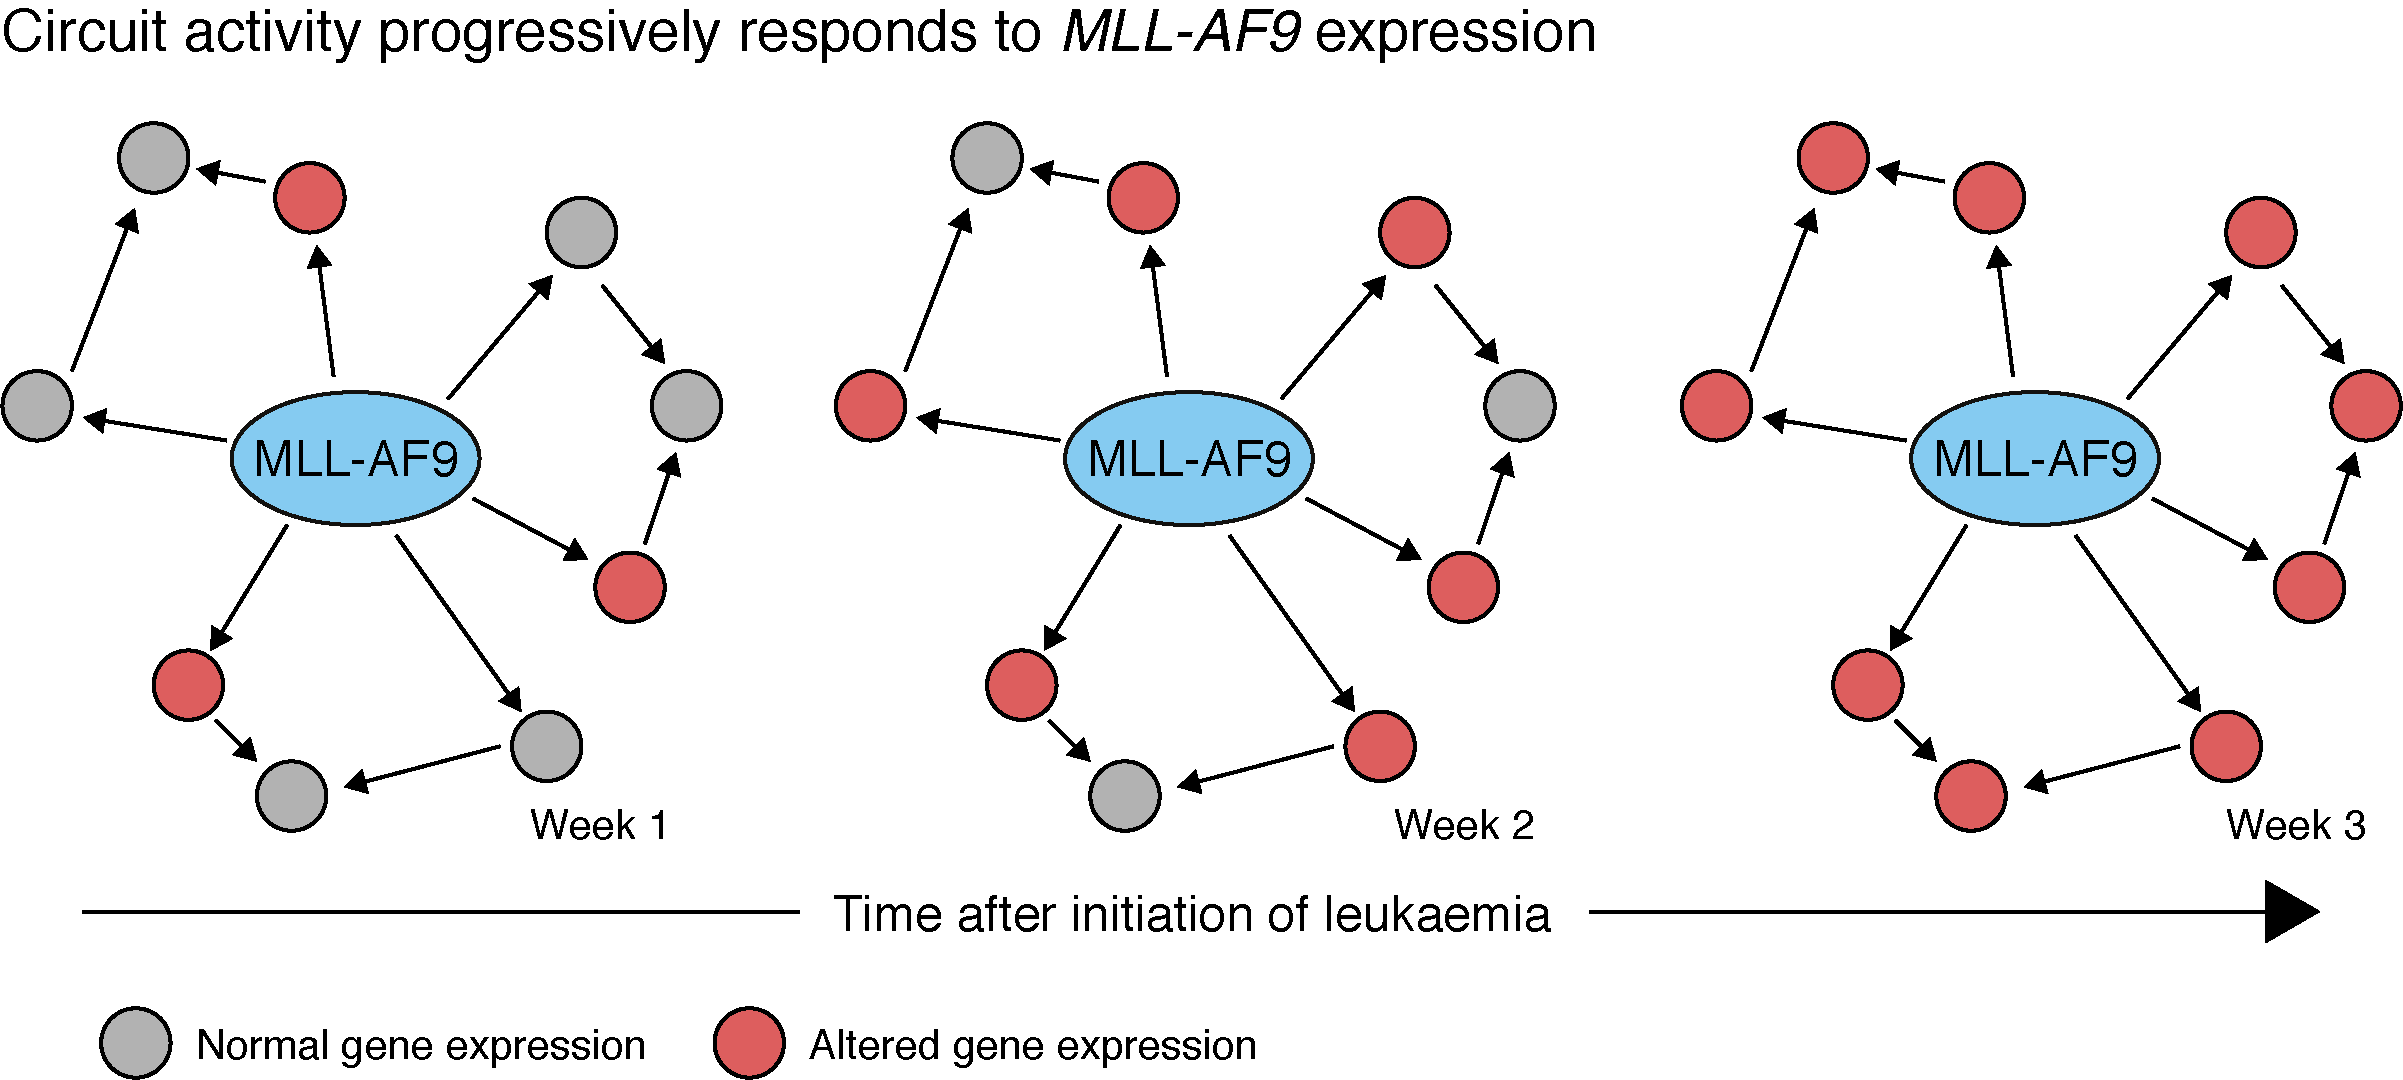
\includegraphics[width=\textwidth,height=\textheight,keepaspectratio]{figures/models/ch5_model-time.png}
    \caption[{Summary model of how circuit activity progressively changes in response to MLL-AF9.}]
    {\textbf{Summary model of how circuit activity progressively changes in response to MLL-AF9.}
    A model illustrating how the TF network progressively responds to \textit{MLL-AF9} expression over time. MLL-AF9 binding is stable at an early time point, and does not change further. Gene expression changes occur subsequent to MLL-AF9 binding, and continues to change over time. This suggests that transcriptional networks may gradually adapt their activity to the fusion protein, as opposed an immediate transformation of a normal GMP network.
    }
    \label{fig:ch5_model-time}
\end{figure}

The methodology used to construct the GRN model of MLL-AF9 GMP leukaemogenesis (section \ref{ch5:grn}) was established using lessons learnt from the construction of the EHT GRN (chapter \ref{chapter3_EHT}) and MLL-AF4 GRN (chapter \ref{chapter4_MA4}). First, ChIPmentation data was used to identify H3K27 acetylation, and thus improves confidence that DAEs are enhancers \citep{heintzman_histone_2009, heintzman_distinct_2007, creyghton_histone_2010}. Additionally, as opposed to relying on motif analysis, MLL-N ChIPmentation was used to evidence MLL-AF9 binding, though the ChIPmentation quality can be further improved with additional sequencing. The identification of E-P interactions in the EHT GRN used a basic approach by annotating accessible elements to the nearest differentially expressed promoter. In this chapter I built upon this method with an iterative approach that allowed for multiple E-P links for each enhancer. This method used an annotation window that expanded with each window until enhancer elements were sufficiently annotated, which allowed for genomic-context dependent annotation. Enhancers within gene dense regions would be sufficiently annotated in a smaller window than enhancers in gene sparse regions, preventing over annotation. As with the EHT GRN, upstream regulators were inferred by motif analysis, and E-P links and predicted TF:target interactions were filtered on the basis of correlation. While the GRN model is not a perfect reflection of MLL-AF9 GMP biology, in particular due to the reliance on TF motifs, these steps improved the robustness of the GRN model for this chapter.

It is important to note that the MLL-AF9 GMP GRN model does not capture any data prior to the W1 time point. It is very likely that considerable effects would be seen by W1. However, the lack of transcriptional divergence between \mybwt{} and \mybmre{} samples until W2 indicate that the time frame for this experiment captures a window of dynamic GRN adaptation. Generating additional RNA-seq and ATAC-seq data on baseline GMPs would improve the study, and allow comparisons with a normal GMP state. An additional consideration, is that the core consensus motif for Myb is small (5'-AACNG-3'), and as such frequently appears throughout the genome and may result in false-positive results. Therefore, the GRN model would benefit from additional Myb ChIPmentation data that would remove the reliance on motif analysis

The \textit{Myc} gene is generally important across leukaemias, and as noted in chapter 4 (section \ref{ch4:essential}, p.\pageref{ch4:essential}) is essential in both MLL-AF4 and MLL-AF9 leukaemias. Further analyses in chapter 4 highlighted cooperation between RUNX1 and MYB to upregulate \textit{Myc} expression (section \ref{ch4:tf-cointeraction}, p.\pageref{ch4:tf-cointeraction}). In the MLL-AF9 GMP GRN model \textit{Myc} expression is not upregulated until W3 (section \ref{ch5:myc}, Fig. \ref{fig:ch5_myc-regulation}), contrary to most genes which are upregulated at W2. As MLL-AF9 binding does not vary, this is likely due to the activation of TFs. Interestingly, while \textit{Myb} expression is well correlated with \textit{Myc}, \textit{Runx1} is instead anti-correlated. The lack of strongly correlated upstream regulators suggests that the W3 \textit{Myc} upregulation is driven by the activation of multiple TFs.

The observation that \textit{Runx1} is anti-correlated with \textit{Myc} expression highlights a striking difference between the MLL-AF4 ALL GRN and MLL-AF9 GMP GRN, in that Runx1 activity appears to be different. While Runx1 activates \textit{Myc} in MLL-AF4 ALL, it may repress \textit{Myc} in MLL-AF9 GMPs. This has been observed in a study from \cite{simeoni_enhancer_2021}, who propose that RUNX1 mediates \textit{MYC} repression in AML by cooperating with FOXC3 to recruit a FOXC3/RUNX1/HDAC1/TLE3 repressor complex. This could be indicative of a general difference in Runx1 activity between myeloid and lymphoid lineages, or that this activity could be specific AML. It remains unclear as to whether Runx1 is a repressive TF genome wide, or if it shows context-dependent regulatory logic. As Myb frequently co-interacts with Runx1 in both the MLL-AF4 GRN (section \ref{ch4:tf-cointeraction}, p.\pageref{ch4:tf-cointeraction}) and the MLL-AF9 GMP GRN (section \ref{ch5:co-interact}, Fig. \ref{fig:ch5_co-interaction}), it is possible that Myb binding alters the regulatory logic of Runx1. This question is difficult to address without \textit{Runx1} perturbation data, but it appears that genes predicted to be regulated by both Myb and Runx1 together are more sensitive to \textit{Myb} perturbation (\mybmre{}) than genes predicted to be regulated by Myb alone (section \ref{ch5:myb-runx1-essential}, Fig. \ref{fig:ch5_myb-runx1-wt-mre}). As such, it is possible that Runx1 supports the activity of Myb, though this hypothesis is as yet untested.

The GRN model was used to probe how Myb drives gene expression changes, and how Myb overexpression is important for leukaemic maintenance \citep{zuber_integrated_2011} (section \ref{ch5:myb-runx1-essential}, Fig. \ref{fig:ch5_essential-targets}). Using differential expression between the \mybwt{} and \mybmre{} genotypes, in combination with \textit{Myb} transcription correlation, \textit{Hoxa11} and \textit{Bcat1} were picked out as two example genes that are strongly downregulated in \mybmre{} samples, and are well-correlated with \textit{Myb} expression. Myb driven upregulation of \textit{Bcat1} could be an important interaction in MLL-AF9 leukaemias, as \textit{Bcat1} overexpression is associated with poor AML prognosis, and is known to drive DNA hypermethylation similar to IDH\textsuperscript{mut} AML \citep{raffel_bcat1_2017}. Myb targets sensitive to \textit{Myb} perturbation (\mybmre{}) were also screened against DepMap gene essentiality data (essentiality in THP-1 cells, \cite{meyers_computational_2017, doench_optimized_2016}), and strikingly, all essential Myb targets were highly correlated with \textit{Myb} expression (R > 0.8). This gene expression correlation suggests that Myb activity is tightly associated with the expression of these essential factors, and the statistical comparison between \mybwt{} and \mybmre{} genotypes suggests this relationship is functional. An essential target of particular relevance is \textit{NAT10}, which is a known AML oncogene associated with poor prognosis, and upon perturbation leads to endoplasmic reticulum stress and apoptosis in AML \citep{zi_targeting_2020, liang_nat10_2020}. These analyses position Myb as an important TF that drives regulation of multiple critical genes in the MLL-AF9 GRN.






